\documentclass[12pt]{article}
\usepackage[utf8]{inputenc}
\usepackage{graphicx}
\usepackage{float}
\usepackage{amsmath}
\usepackage{placeins}
\usepackage{gensymb}



\usepackage[letterpaper,margin=0.75in]{geometry}
\graphicspath{images/}
\begin{document}
\begin{titlepage}
\begin{center}
% Upper part of the page
\vbox{}
\vbox{}
\vbox{}
\vbox{}
\vbox{}
\vbox{}
\vbox{}
\vbox{}
\vbox{}
\vbox{}
\vbox{}
\vbox{}

\includegraphics[width=0.75\textwidth]{Images/ubc.png}\\[0.5cm]
\textrm{Martin Alejo}\\[0.5cm]
\catcode`#=12
\textrm{#75296665}\\[0.5cm]
\textrm{October 28, 2022}\\[0.5cm]
\textrm{Mini Project 2}\\[0.5cm]
\textrm{University of British Columbia}\\[0.5cm]
\textrm{Electrical and Computer Engineering}\\[0.5cm]
\textrm{ELEC 301}\\[0.5cm]
\textrm{Instructor: Nicolas Jaeger}\\[0.5cm]
\vbox{ }
\end{center}
\end{titlepage}
\pagebreak
\pagenumbering{roman}
\tableofcontents
\pagebreak
\listoffigures
\listoftables
\pagebreak
\pagenumbering{arabic}
\section{Introduction}
In this project, we will be using NI $Mulitsim^{TM}$ to simulate various transistors, measuring simulated values. We will also be calculating their respective theoretical values and comparing them with the simulated. We will also be assuming that $V_T=0.025V$
\section{Part 1}
\subsection{Part a)}
From the datasheet, we can see that the small signal parameters of the 2N3904 transistor for $V_{ce}= 10V, I_c = 1mA, f=1kHz,T =  25^oC$ is as follows:  

\begin{table}[h!]
\centering
\begin{tabular}{|c c c c| }
 \hline
    & Min & Max & Unit \\
    \hline\hline
$h_{fe}$ & 100 & 400 & -\\
$h_{ie}$ & 1   & 10  & k$\Omega$\\
$h_{oe}$ & 1   & 40 & $\mu mho$\\
 \hline
\end{tabular}
\caption{Small Signal Values from Data Sheet}
\label{table:small signal}
\end{table}

For this lab however, we will be using the average of those values. Therefore:
\begin{center}
$h_{fe} =250, h_{ie} = 5.5 , h_{oe} = 20.5$
\end{center}

\subsection{Part b)}

Figure \ref{fig:ibvbeib}, Figure \ref{fig:icvceib} and Figure \ref{fig:icvcevbe} below shows $I_b$ vs $V_{be}$,$I_c$ vs $V_{ce}$ and $I_c$ vs $V_{be}$ respectively.
\begin{figure}[H]
\centering
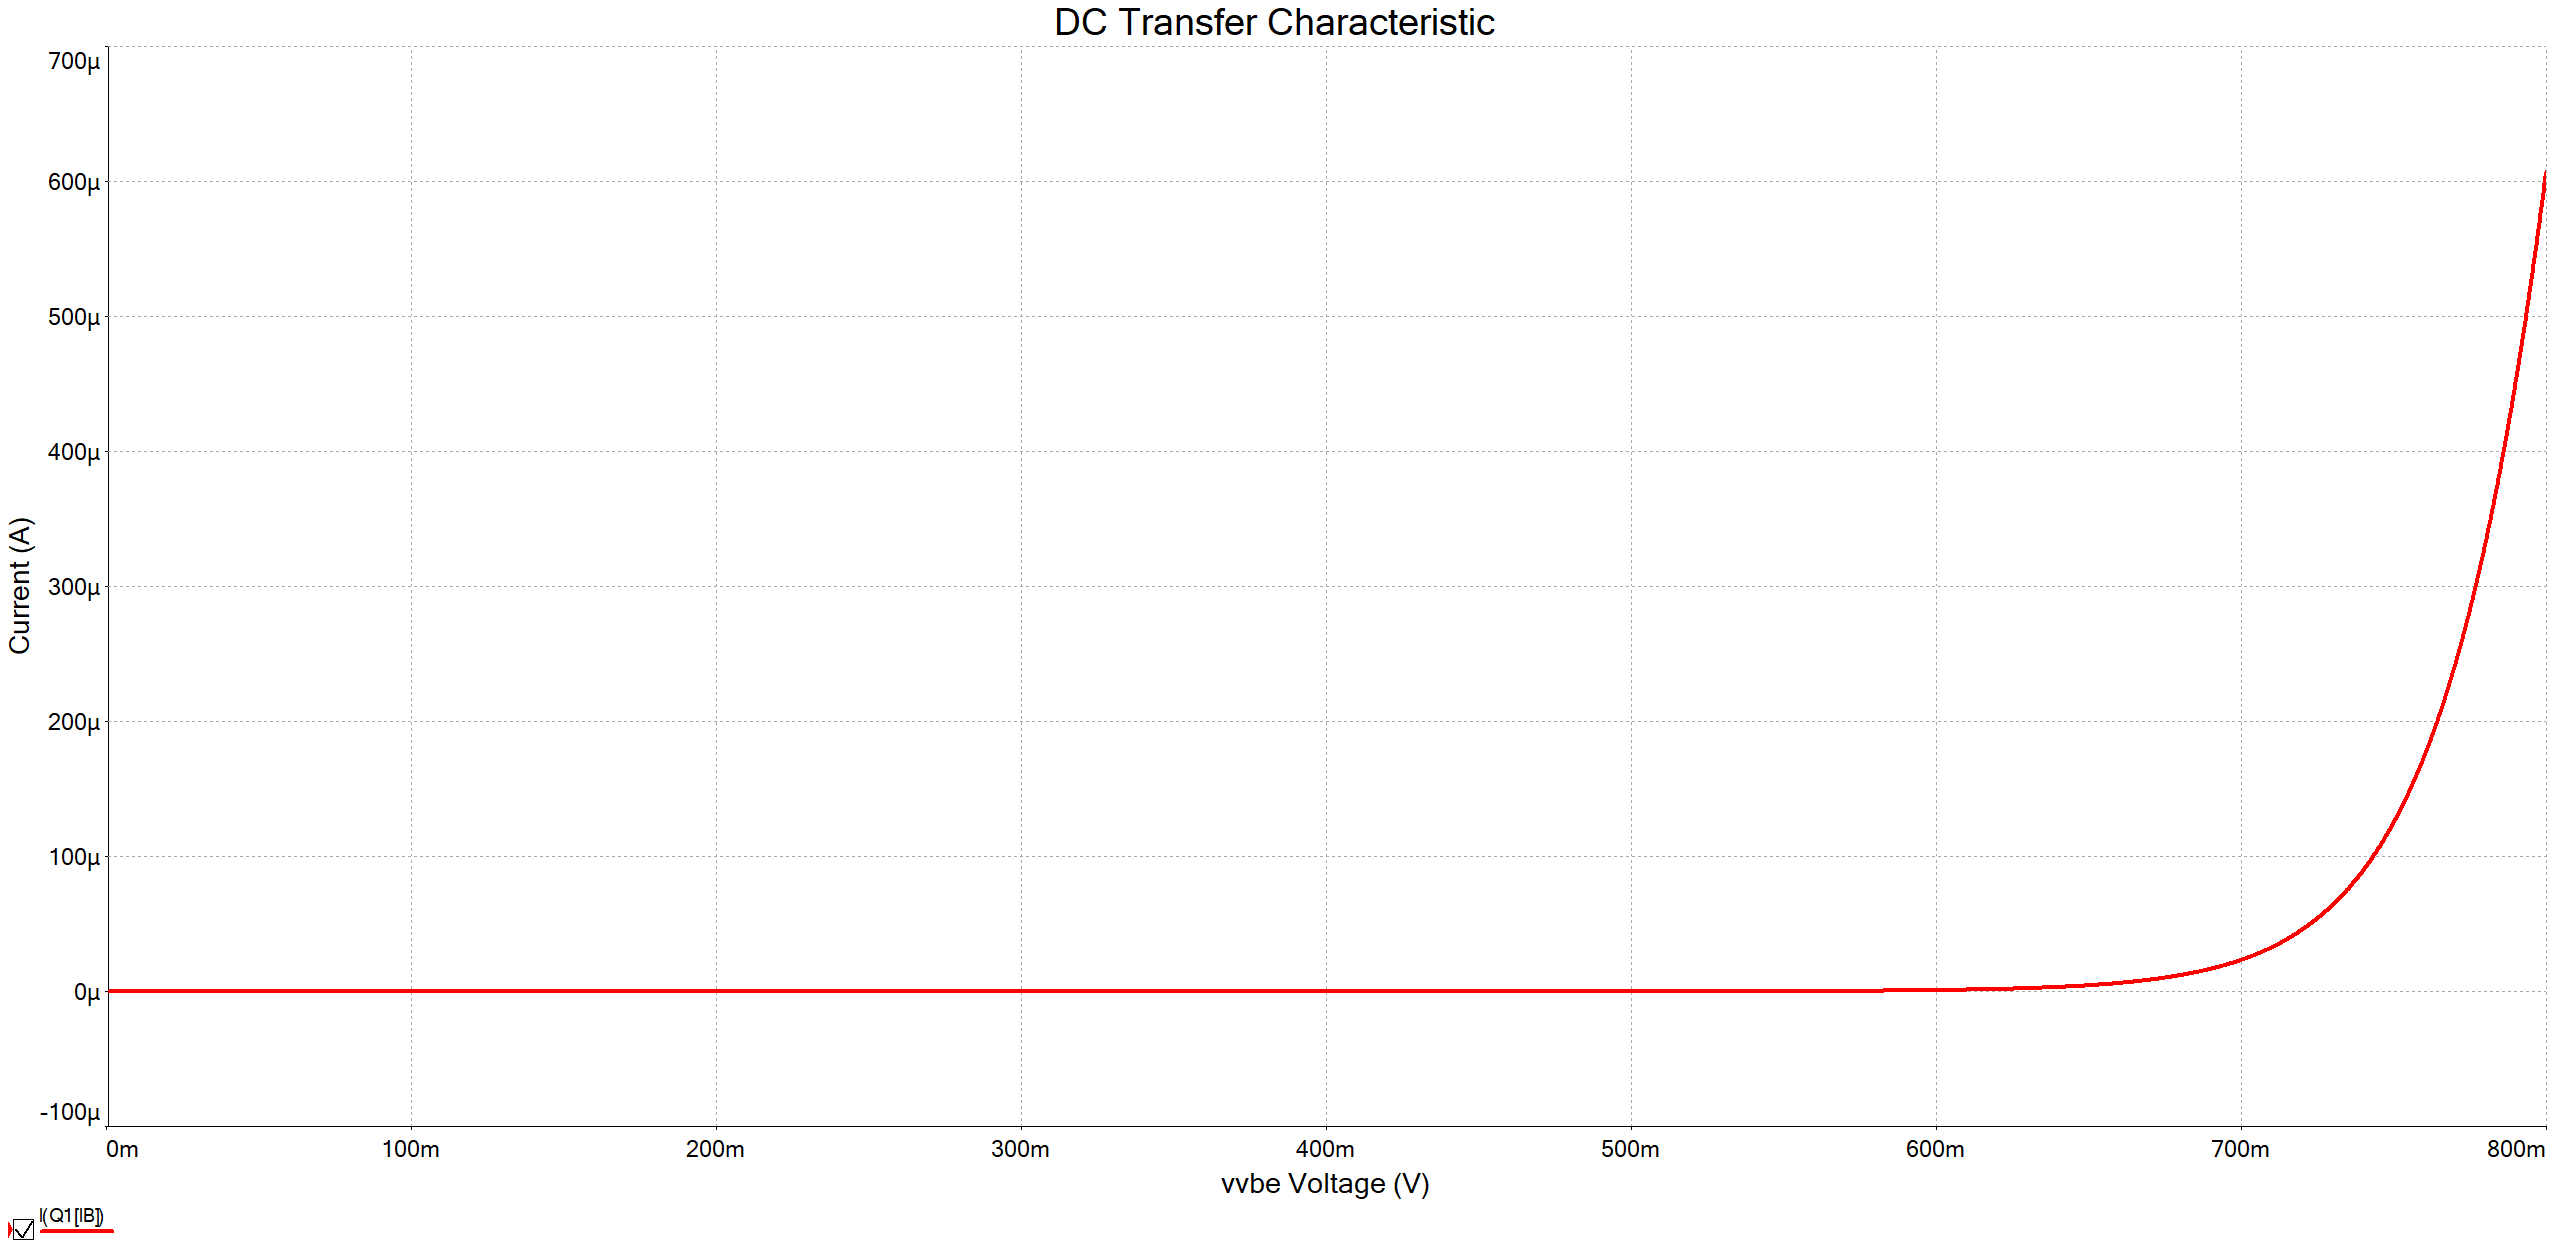
\includegraphics[width=0.75\textwidth]{Images/Ib_vs_Vbe.png}\\
\caption{$I_b$ vs $V_{be}$}
\label{fig:ibvbeib}
\end{figure}
The DC sweep of this simulation is about 0V to 2V in 0.01V increments.
\begin{figure}[H]
\centering
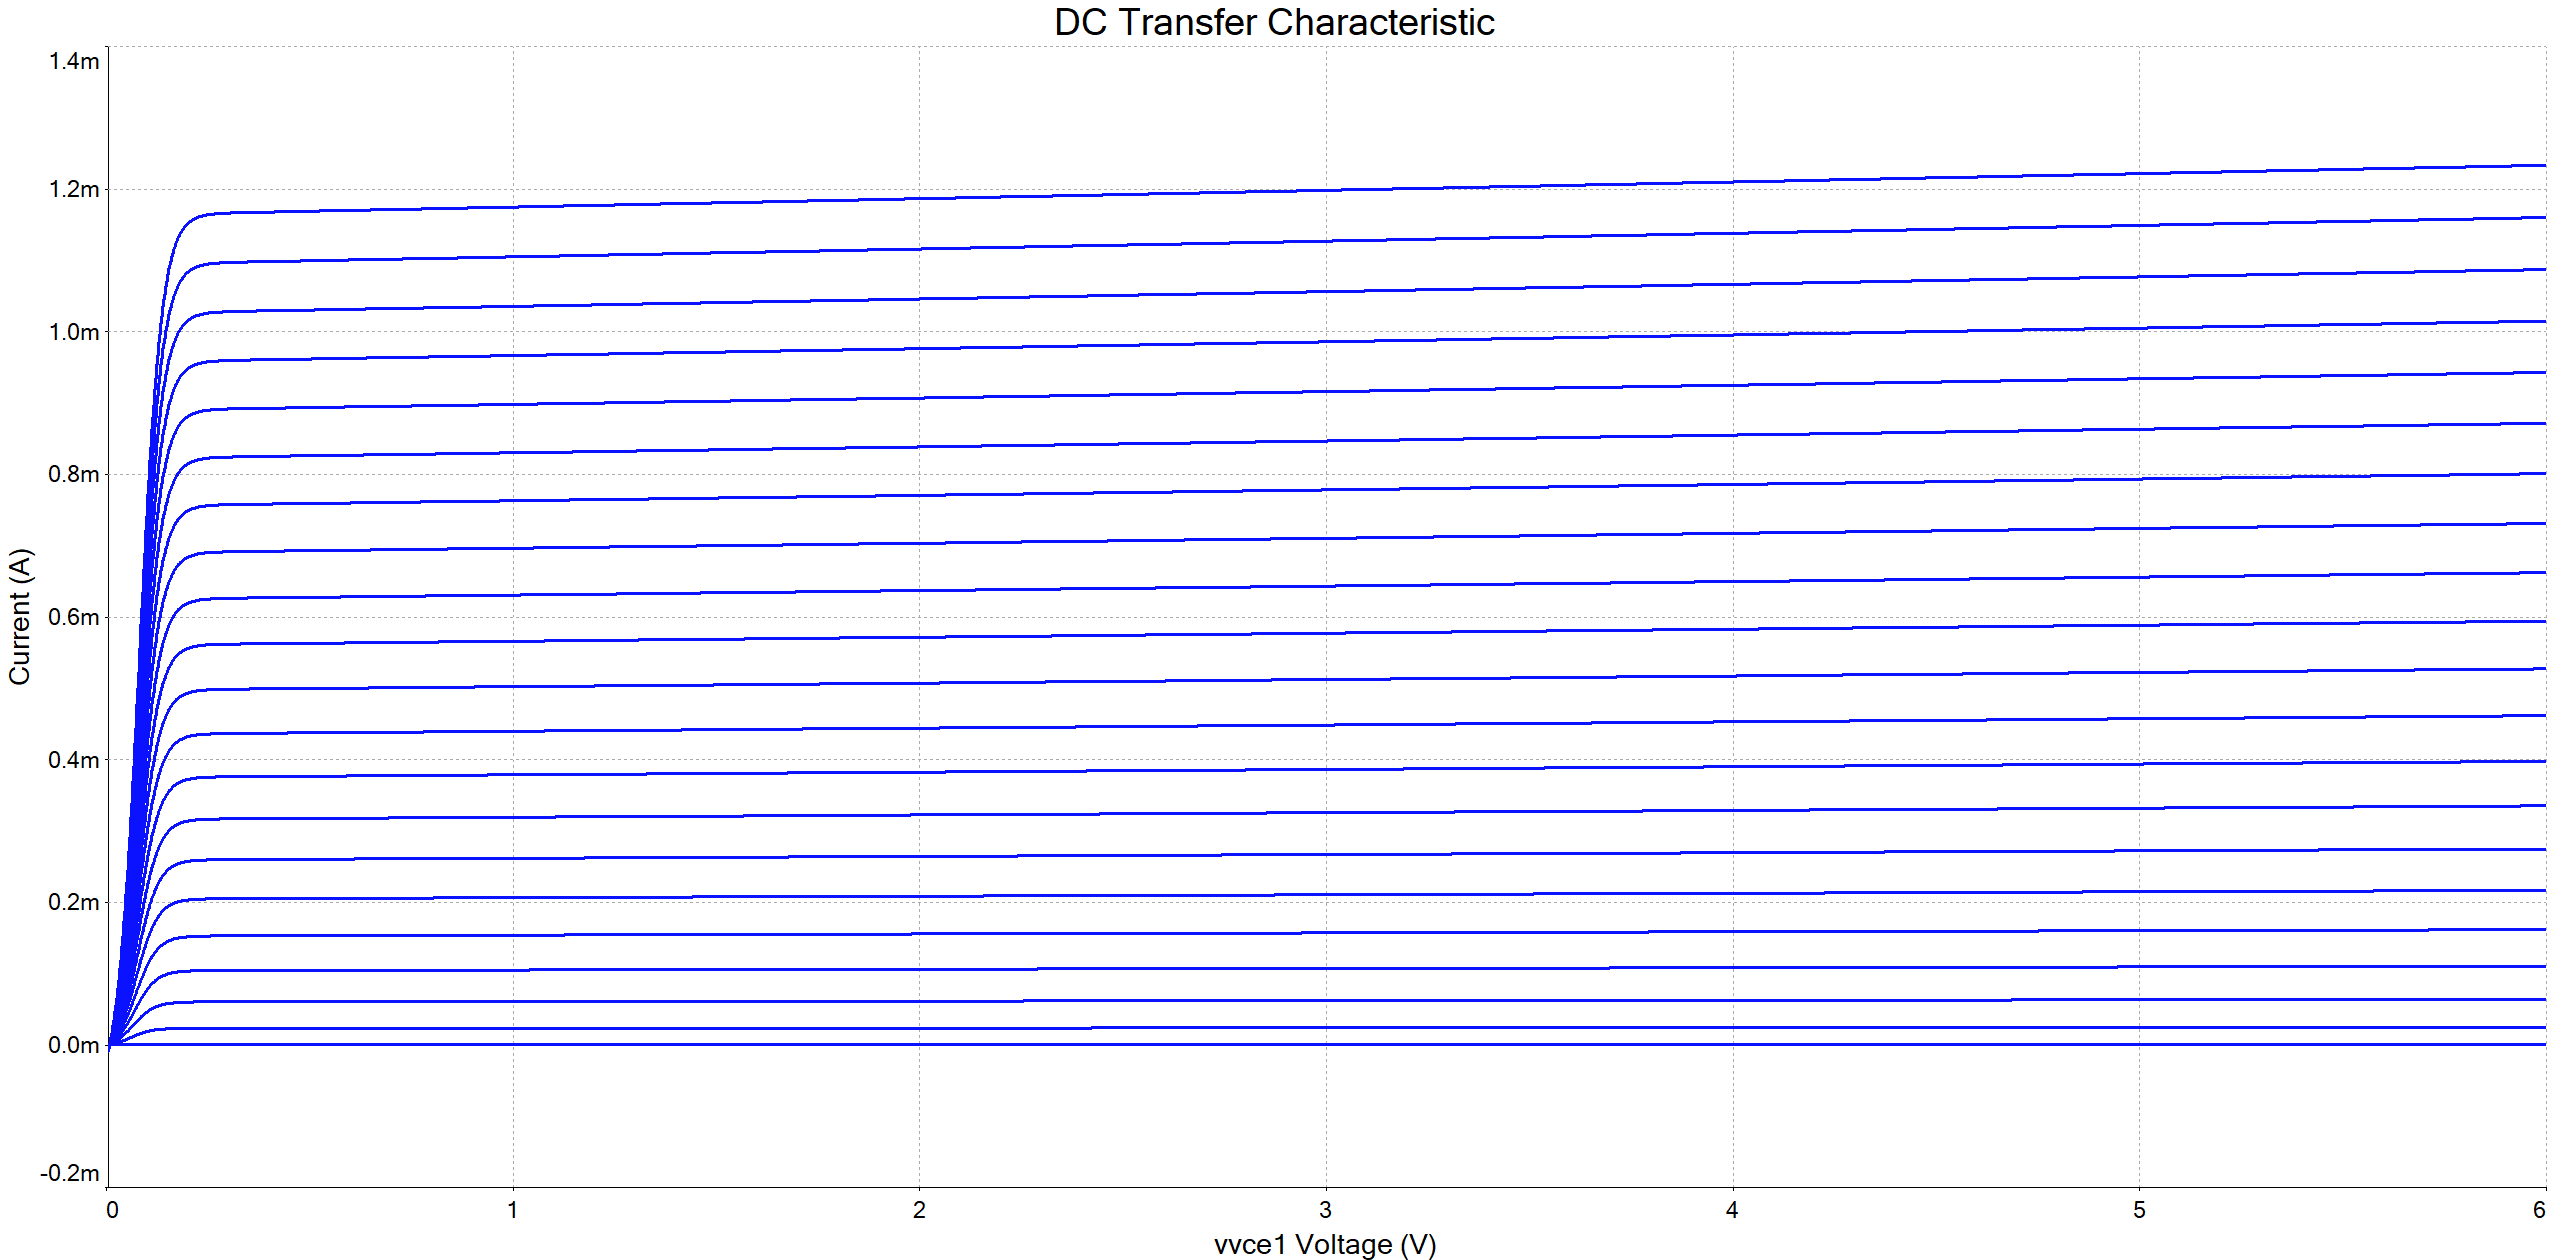
\includegraphics[width=0.75\textwidth]{Images/Ic_vs_Vce.png}\\
\caption{$I_c$ vs $V_{ce}$, varying $I_b$}
\label{fig:icvceib}
\end{figure}
The DC sweep of this simulation is $V_{ce}$ from 0 to 6V with 1mV step and $I_b$ from 0A to 10$\mu$A with $0.5\mu$A step. From this graph, we can determine the value of $I_c$ and from there, since $\beta= \frac{I_c}{I_b}$. From using the cursor tool, we can find that when $I_c=1m$A and $V_{ce}$=5V, we can see that $I_b$=$8.5\mu$A. Following the calculation that was stated previously, we can estimate that:
\newline
\begin{center}
$\beta= \frac{I_c}{I_b}$=$\frac{1*10^{-3}}{8.5*10^{-6}}$= \boxed{117}
\end{center}
\begin{figure}[H]
\centering
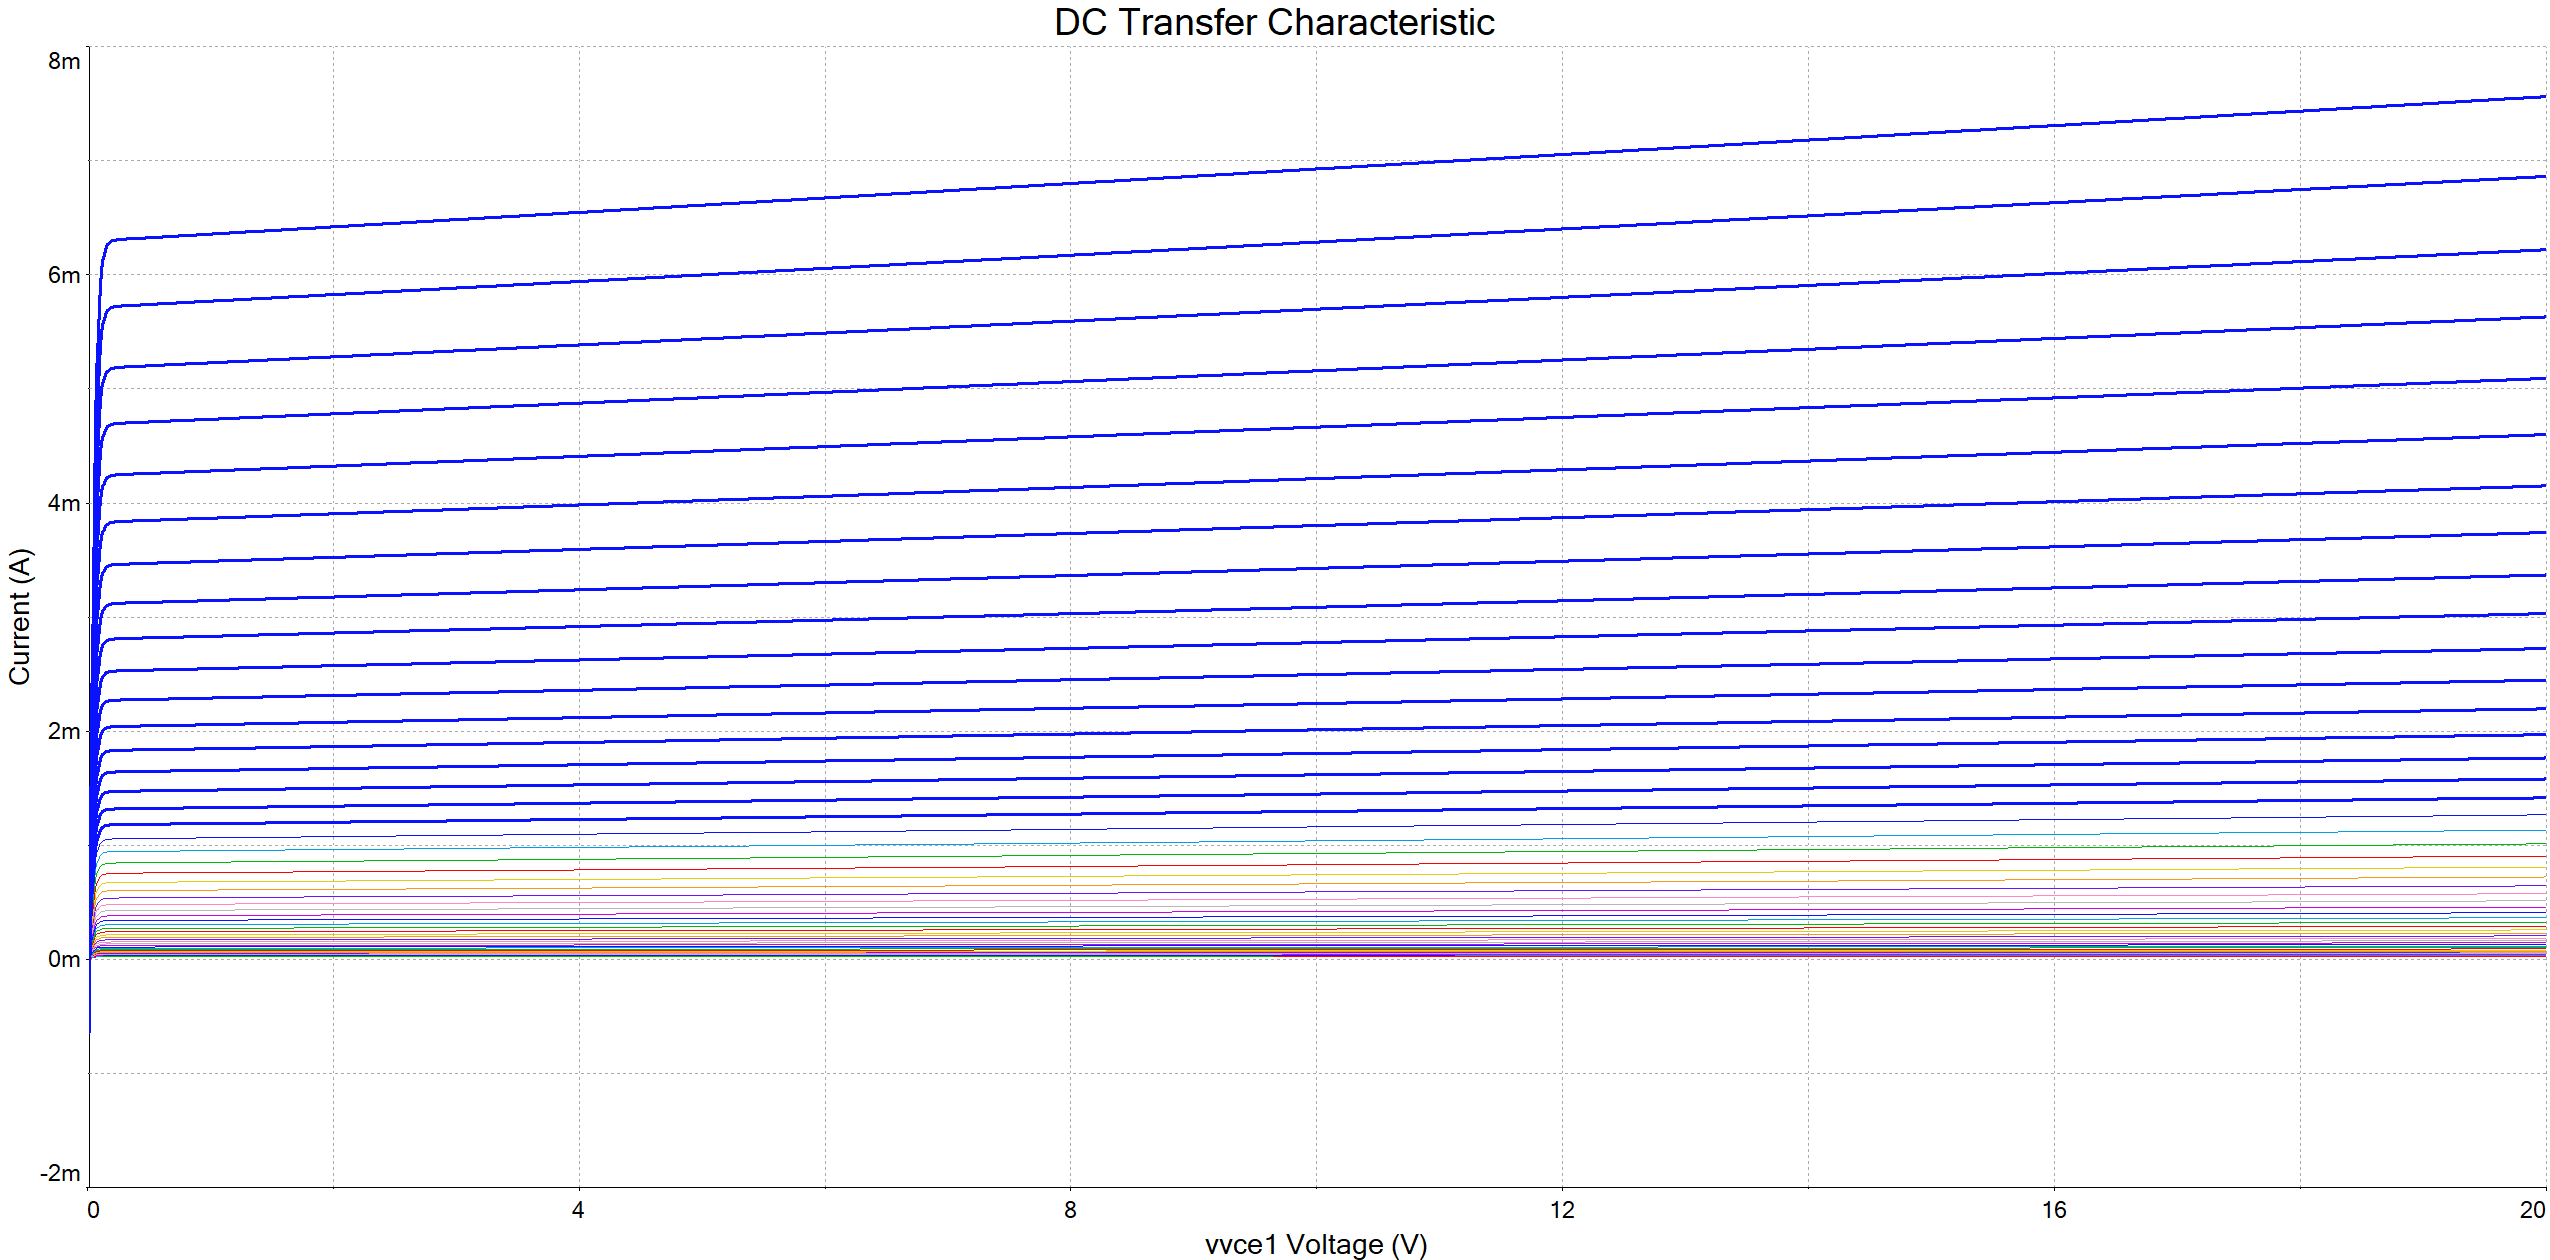
\includegraphics[width=0.75\textwidth]{Images/ic__vs_vce_vbe.png}
\caption{$I_c$ vs $V_{ce}$, varying $V_{be}$}
\label{fig:icvcevbe}
\end{figure}
The DC sweep of this simulation is $V_{ce}$ from 0 to 20V with 1mV step and $V_{be}$ from 0.55V to 0.7V with 3mA step. From the graph, when we set $V_{ce}$ = 5V and $I_c$=1mA, we can find using the cursor tool in $Multisim^{TM}$ that $V_{be}$=0.646. To find the Early Voltage ($V_A$) we can use Figure \ref{fig:icvcevbe}. Using the top-most line ($V_{be}=0.7$), we can use the slope of the linear part of that trace and find the x-intercept. The resulting x-intercept will be $V_A$. Here we can use the equation of the line to find the x-intercept, selecting two arbitrary points on that trace as $x_1$ and $y_1$:
\begin{center}
    $6.4192*10^{-3}$-y=$63.3687*10^{-6}*(x-2)$
\end{center}
setting $y=0$ and finding x, we will find that $-x=V_A$=\boxed{99.299V}
\newline
\newline
To find $r_{\pi}$, $g_m$, and $r_o$:
\begin{center}
    $r_{\pi}=\frac{\beta}{g_m}$, $g_m=\frac{I_c}{V_T}$, and $r_o =\frac{V_A}{I_c}$
\end{center}
Evaluating:
\begin{center}
 $g_m=\frac{1*10^{-3}}{0.025}$ = \boxed{0.04S},$r_{\pi}=\frac{117}{0.04}$ =\boxed{2.941k\Omega}, $r_o =\frac{99.299V}{1*10^{-3}A}$ = \boxed{99.299k\Omega}
\end{center}
\subsubsection{Comparing Values}
Comparing all of the values from the data sheet and the calculated parts, we can see that the $\beta$ value that is calculated is within the range of the minimum and maximum value as stated in the data sheet. The same can be said about the other parts that were calculated.
\subsection{Part c)}
\subsubsection{Part i)}
Finding the values of $R_{B1}$,$R_{B2}$,$R_C$,$R_E$ with:
\begin{center}
    $\beta$=117, $V_{be}=0.646V$, $I_c=1mA$, $V_{cc}=15V$,$V_{ce}=4V$, $R_E=\frac{R_C}{2}$
\end{center}

Using these values and assumptions we can find the value of $R_{C}$ assuming ($R_E=\frac{R_C}{2}$,$V_{CE}=4V$,$V_{CC}=15$) with: 
\begin{center}
$I_E=I_C+\frac{I_C}{\beta}$
\end{center}
\begin{center}
$15=I_c*R_C+4+I_E*\frac{R_C}{2}$ 
\end{center}
\begin{center}
We find that $R_C$=\boxed{7.313k\Omega}, and $R_E$=\boxed{3.656k\Omega}
\end{center}
And we can find $R_{B1}$ and $R_{B2}$ with:
\begin{center}
$\frac{15-V_B}{R_B1}=I_B+\frac{V_B}{R_{B2}}$
\end{center}
\begin{center}
$V_B=15*(\frac{R_{B2}}{R_{B1}+R_{B2}})$    
\end{center}
However, it is not possible for us to solve for $R_{B1}$, and $R_{B2}$. This is because their relationships cannot be solved with a system of linear equations. However what we can do is to estimate their values. We can choose that $R_{B1}$ is about 107k$\Omega$, and following that we can use the equations as stated previously to solve that $R_{B2}$=48.982k$\Omega$.
\subsubsection{Part ii)}
For the 1/3 rule estimation, We will be using the first version of the 1/3 rule. Where we can assume:
\begin{center}
    $V_C=V_{CC}*\frac{2}{3}$, $V_B=V_{CC}*\frac{1}{3}$,$V_{be}=0.7V$ and $I_1=\frac{I_E}{\sqrt{\beta}}$ 
\end{center}
Here is the completed circuit after finding all of the values:
\begin{figure}[H]
\centering
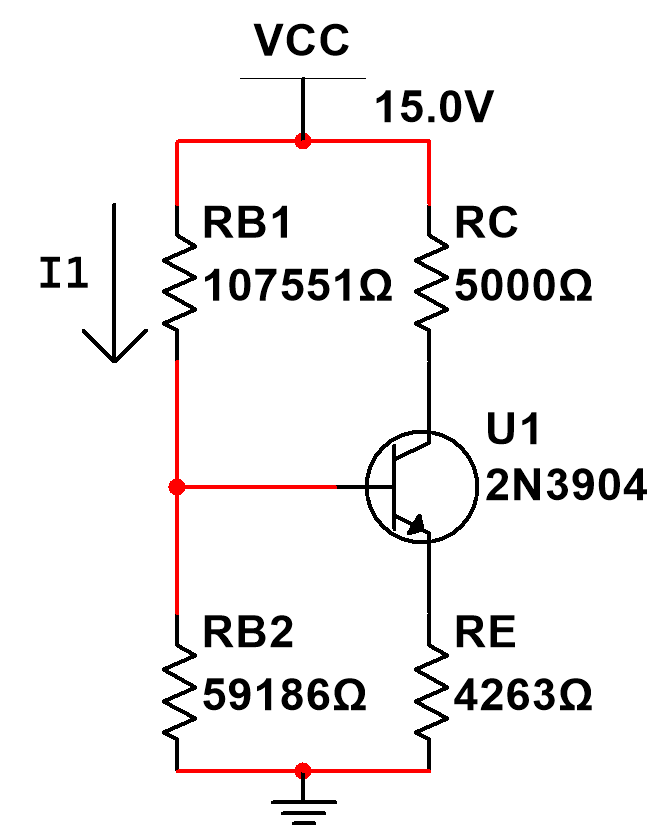
\includegraphics[height=0.25\textwidth]{Images/part1c_circuit.png}\\
\caption{Circuit With Approximated Resistor Values}
\label{fig:part1c}
\end{figure}

Here are the approximated operating points:
\begin{table}[h!]
\centering
\begin{tabular}{|l|l|l|l|l|l|}
\cline{1-6}
$I_C$      & $I_B$      & $I_E$      & $V_C$     & $V_B$     & $V_E$     \\ \cline{1-6}
\hline
1.013mA & 8.513uA & 1.021mA & 9.937V & 4.999V & 4.353V \\ 
\hline
\end{tabular}
\caption{Simulated DC Operating Point(Calculated Resistances)}
\label{table:DC Operating Values}
\end{table}
\subsubsection{Part iii)}
Here we will now design our circuit based on standard resistance values. They were chosen to be:
\begin{center}
    $R_{B1}=110k\Omega$,$R_{B2}=62k\Omega$,$R_{C}=5.1k\Omega$,$R_{E}=4.3k\Omega$
\end{center}
\begin{table}[h!]
\centering
\begin{tabular}{|l|l|l|l|l|l|}
\cline{1-6}
$I_C$      & $I_B$      & $I_E$      & $V_C$     & $V_B$     & $V_E$     \\ \cline{1-6}
\hline
1.019mA & 8.574uA & 1.028mA & 9.801V & 5.07V & 4.42V \\ 
\hline
\end{tabular}
\caption{Simulated DC Operating Point(Standard Resistances)}
\label{table:DC Standard Operating Values}
\end{table}
\subsubsection{Part iv)}
Comparing the DC operating point values from parts i),ii), and iii), we can find that the measured values with standard and calculated resistances are very similar.However, the values from Part i) are not similar to the values that we have estimated in Part ii). We can then conclude that using the $\frac{1}{3}$ rule is very accurate in estimating the resistances needed to bias the BJT.  
\subsection{Part d)}
\FloatBarrier
Here are the measured DC Operating Point values from the 2N2222A and the 2N4401 respectively:

\begin{table}[h!]
\centering
\begin{tabular}{|l|l|l|l|l|l|}
\cline{1-6}
$I_C$      & $I_B$      & $I_E$      & $V_C$     & $V_B$     & $V_E$     \\ \cline{1-6}
\hline
1.053mA & 6.275uA & 1.059mA & 9.629V & 5.158V & 4.556V \\ 
\hline
\end{tabular}
\caption{Simulated DC Operating Point(Standard Resistances, 2N2222A)}
\label{table:DC Standard Operating Values(2N2222A)}
\end{table}

For this transistor below (2N2222A), we find that $\beta$=\boxed{168}. We Also we can see that $r_\pi$=\boxed{3.984k\Omega} and $g_m$=\boxed{0.04}


\begin{table}[h!]
\centering
\begin{tabular}{|l|l|l|l|l|l|}
\cline{1-6}
$I_C$      & $I_B$      & $I_E$      & $V_C$     & $V_B$     & $V_E$     \\ \cline{1-6}
\hline
1.033mA & 6.963uA & 1.04mA & 9.731V & 5.131V & 4.472V \\ 
\hline
\end{tabular}
\caption{Simulated DC Operating Point(Standard Resistances, 2N4401)}
\label{table:DC Standard Operating Values(2N4401)}
\end{table}
\FloatBarrier
For this transistor (2N4401), we find that $\beta$=\boxed{148}. Also we can see that $r_\pi$=\boxed{3.590k\Omega} and $g_m$=\boxed{0.04}

Comparing the two tables to the values from part iii), we can see that while some parts are similar, some other values are completely different. This is because of the different characteristics that each transistor has, as they are all not exactly the same.

\section{Part 2}
\subsubsection{Part a)}
Here is the equivalent Common Emitter Amplifier that we will be using:

\begin{figure}[H]
\centering
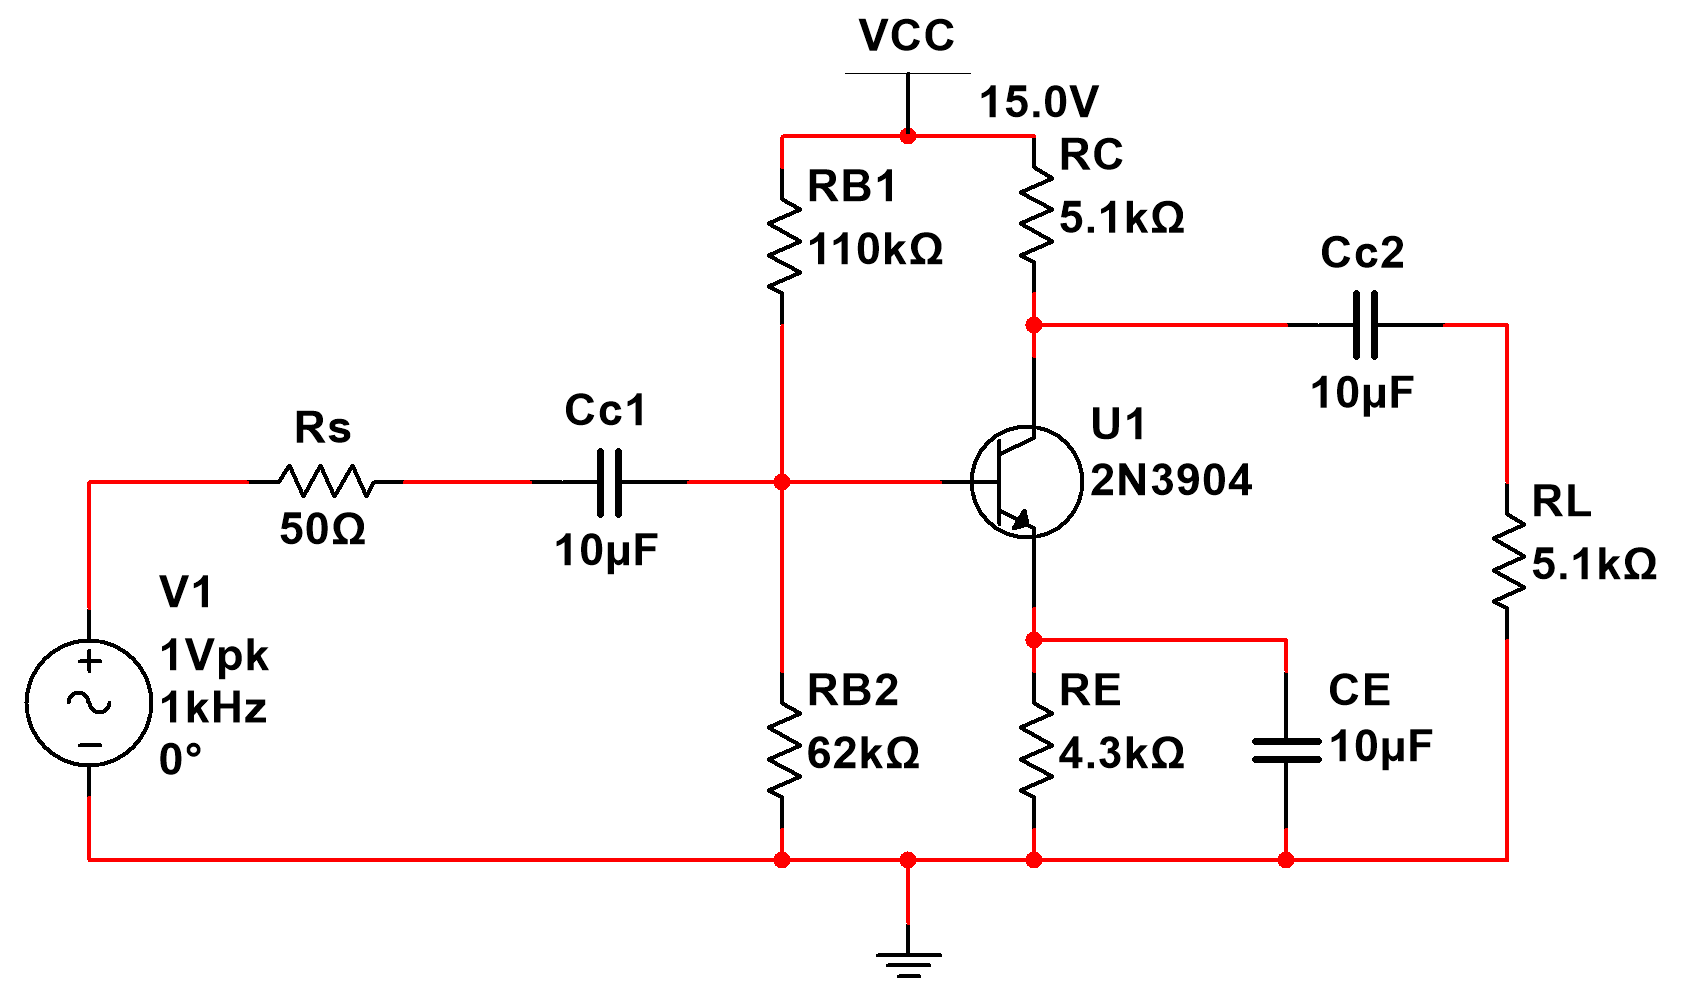
\includegraphics[height=0.40\textwidth]{Images/2acircuit.png}\\
\caption{2N3904 Common Emitter Amplifier}
\label{fig:part2a_circuit}
\end{figure}

Below is our bode and phase plot for this circuit:

\begin{figure}[H]
\centering
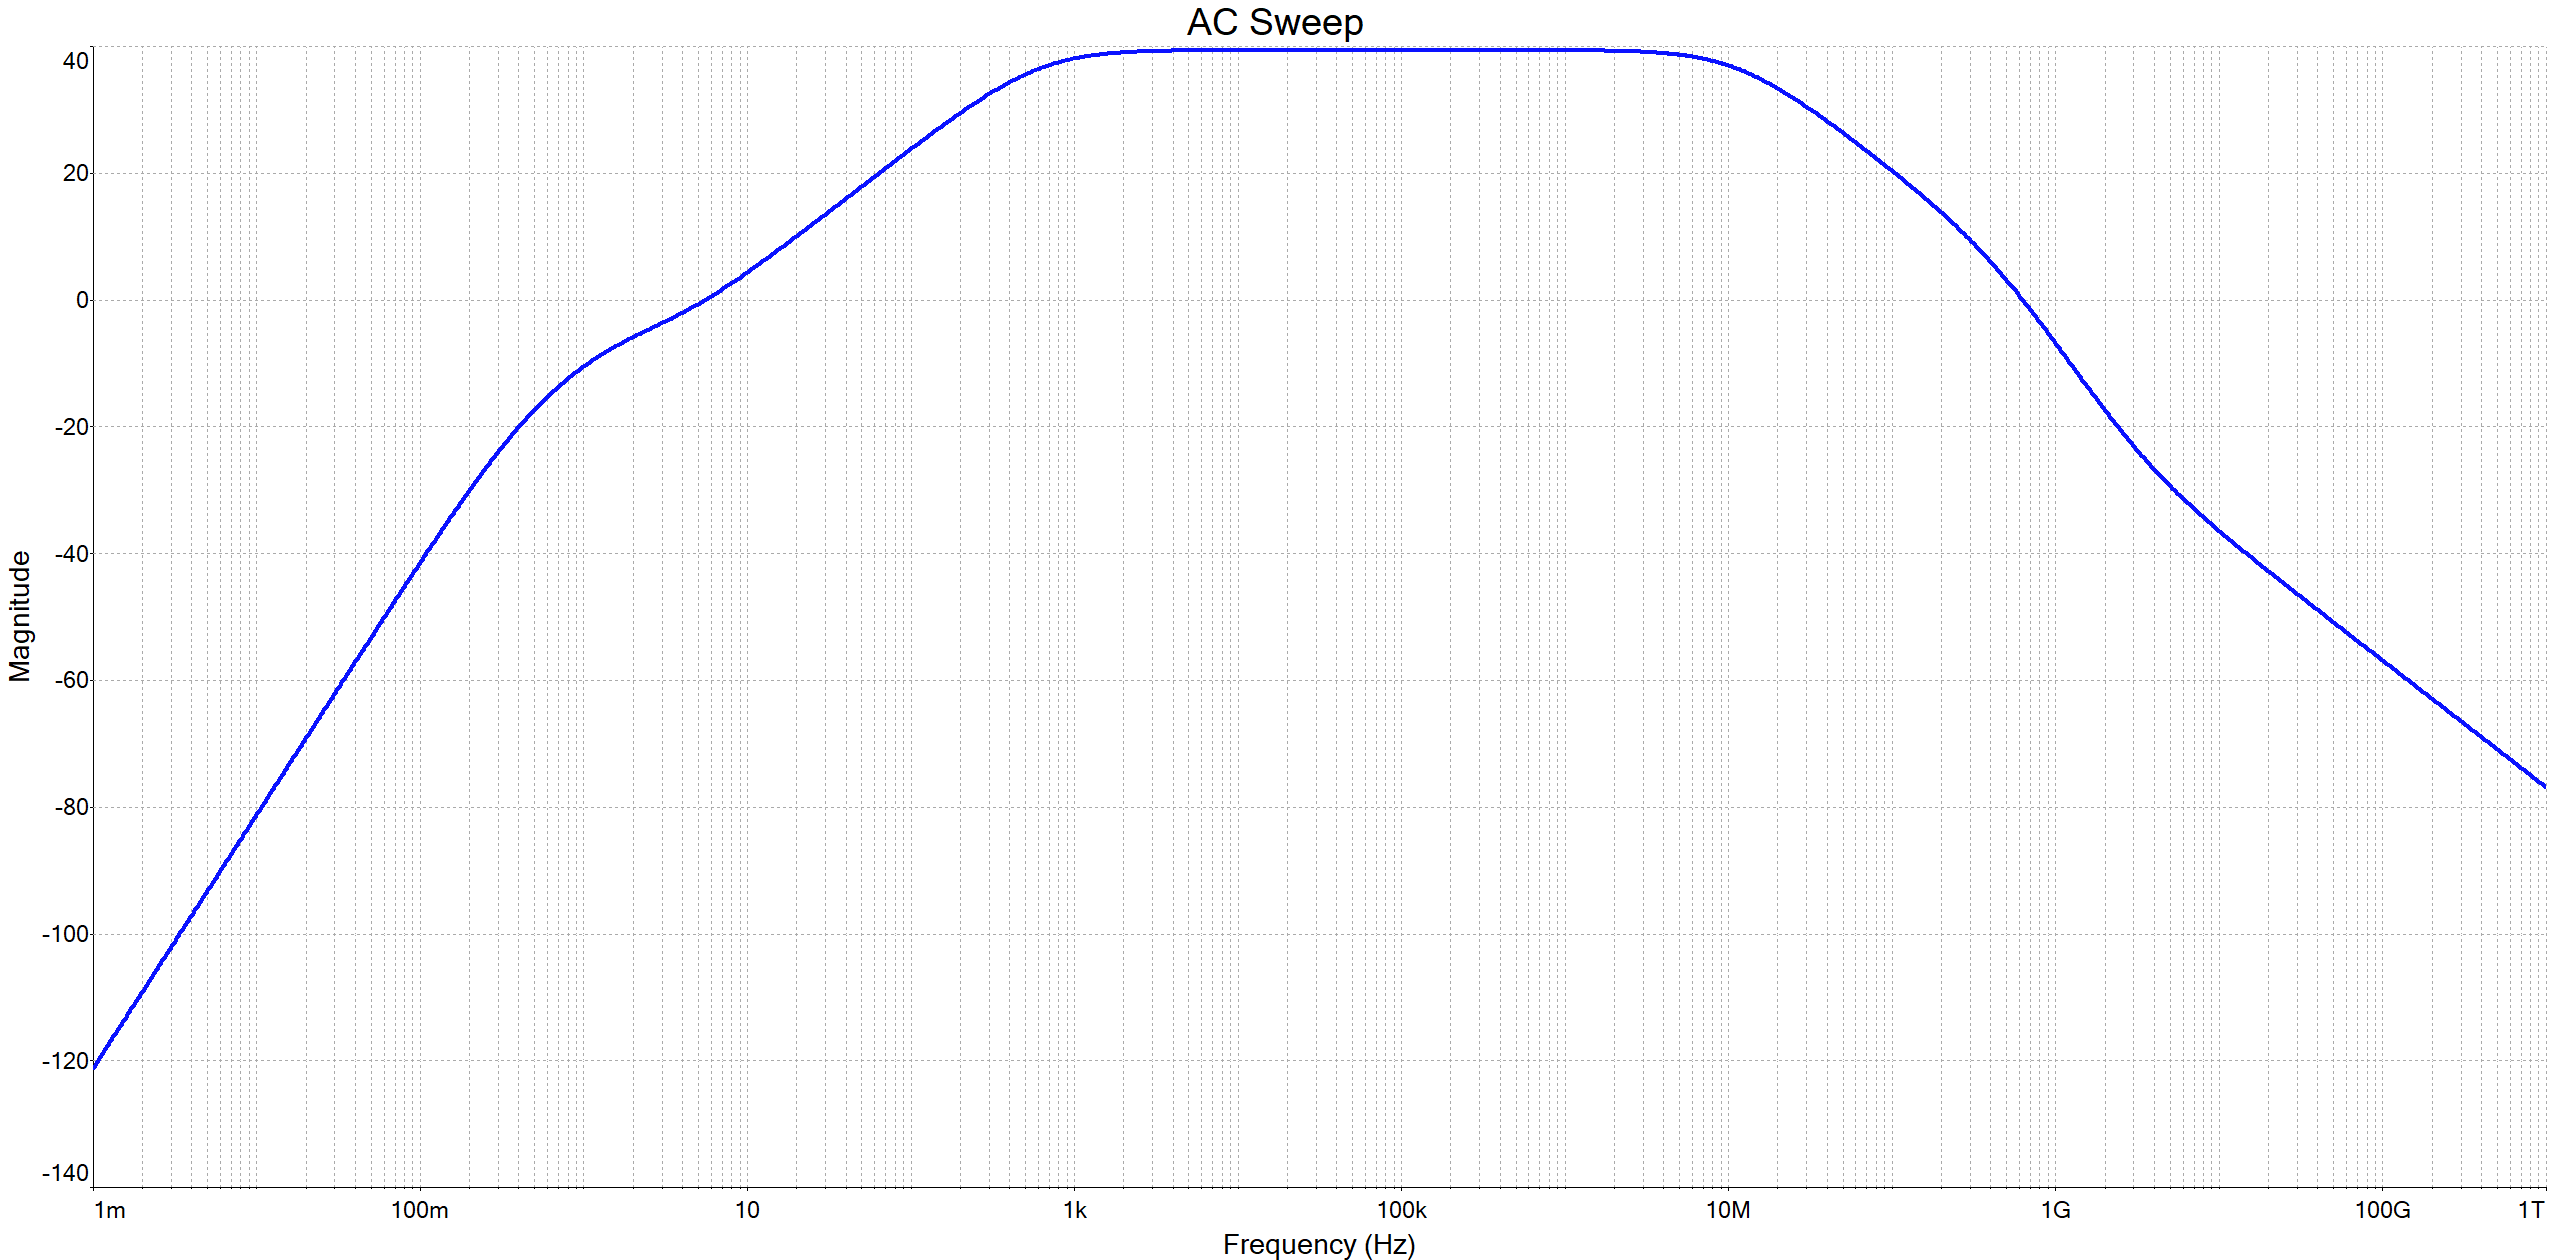
\includegraphics[height=0.45\textwidth]{Images/part2a.png}\\
\caption{2N3904 Bode Plot}
\label{fig:part2a_bodeplot}
\end{figure}

\begin{figure}[H]
\centering
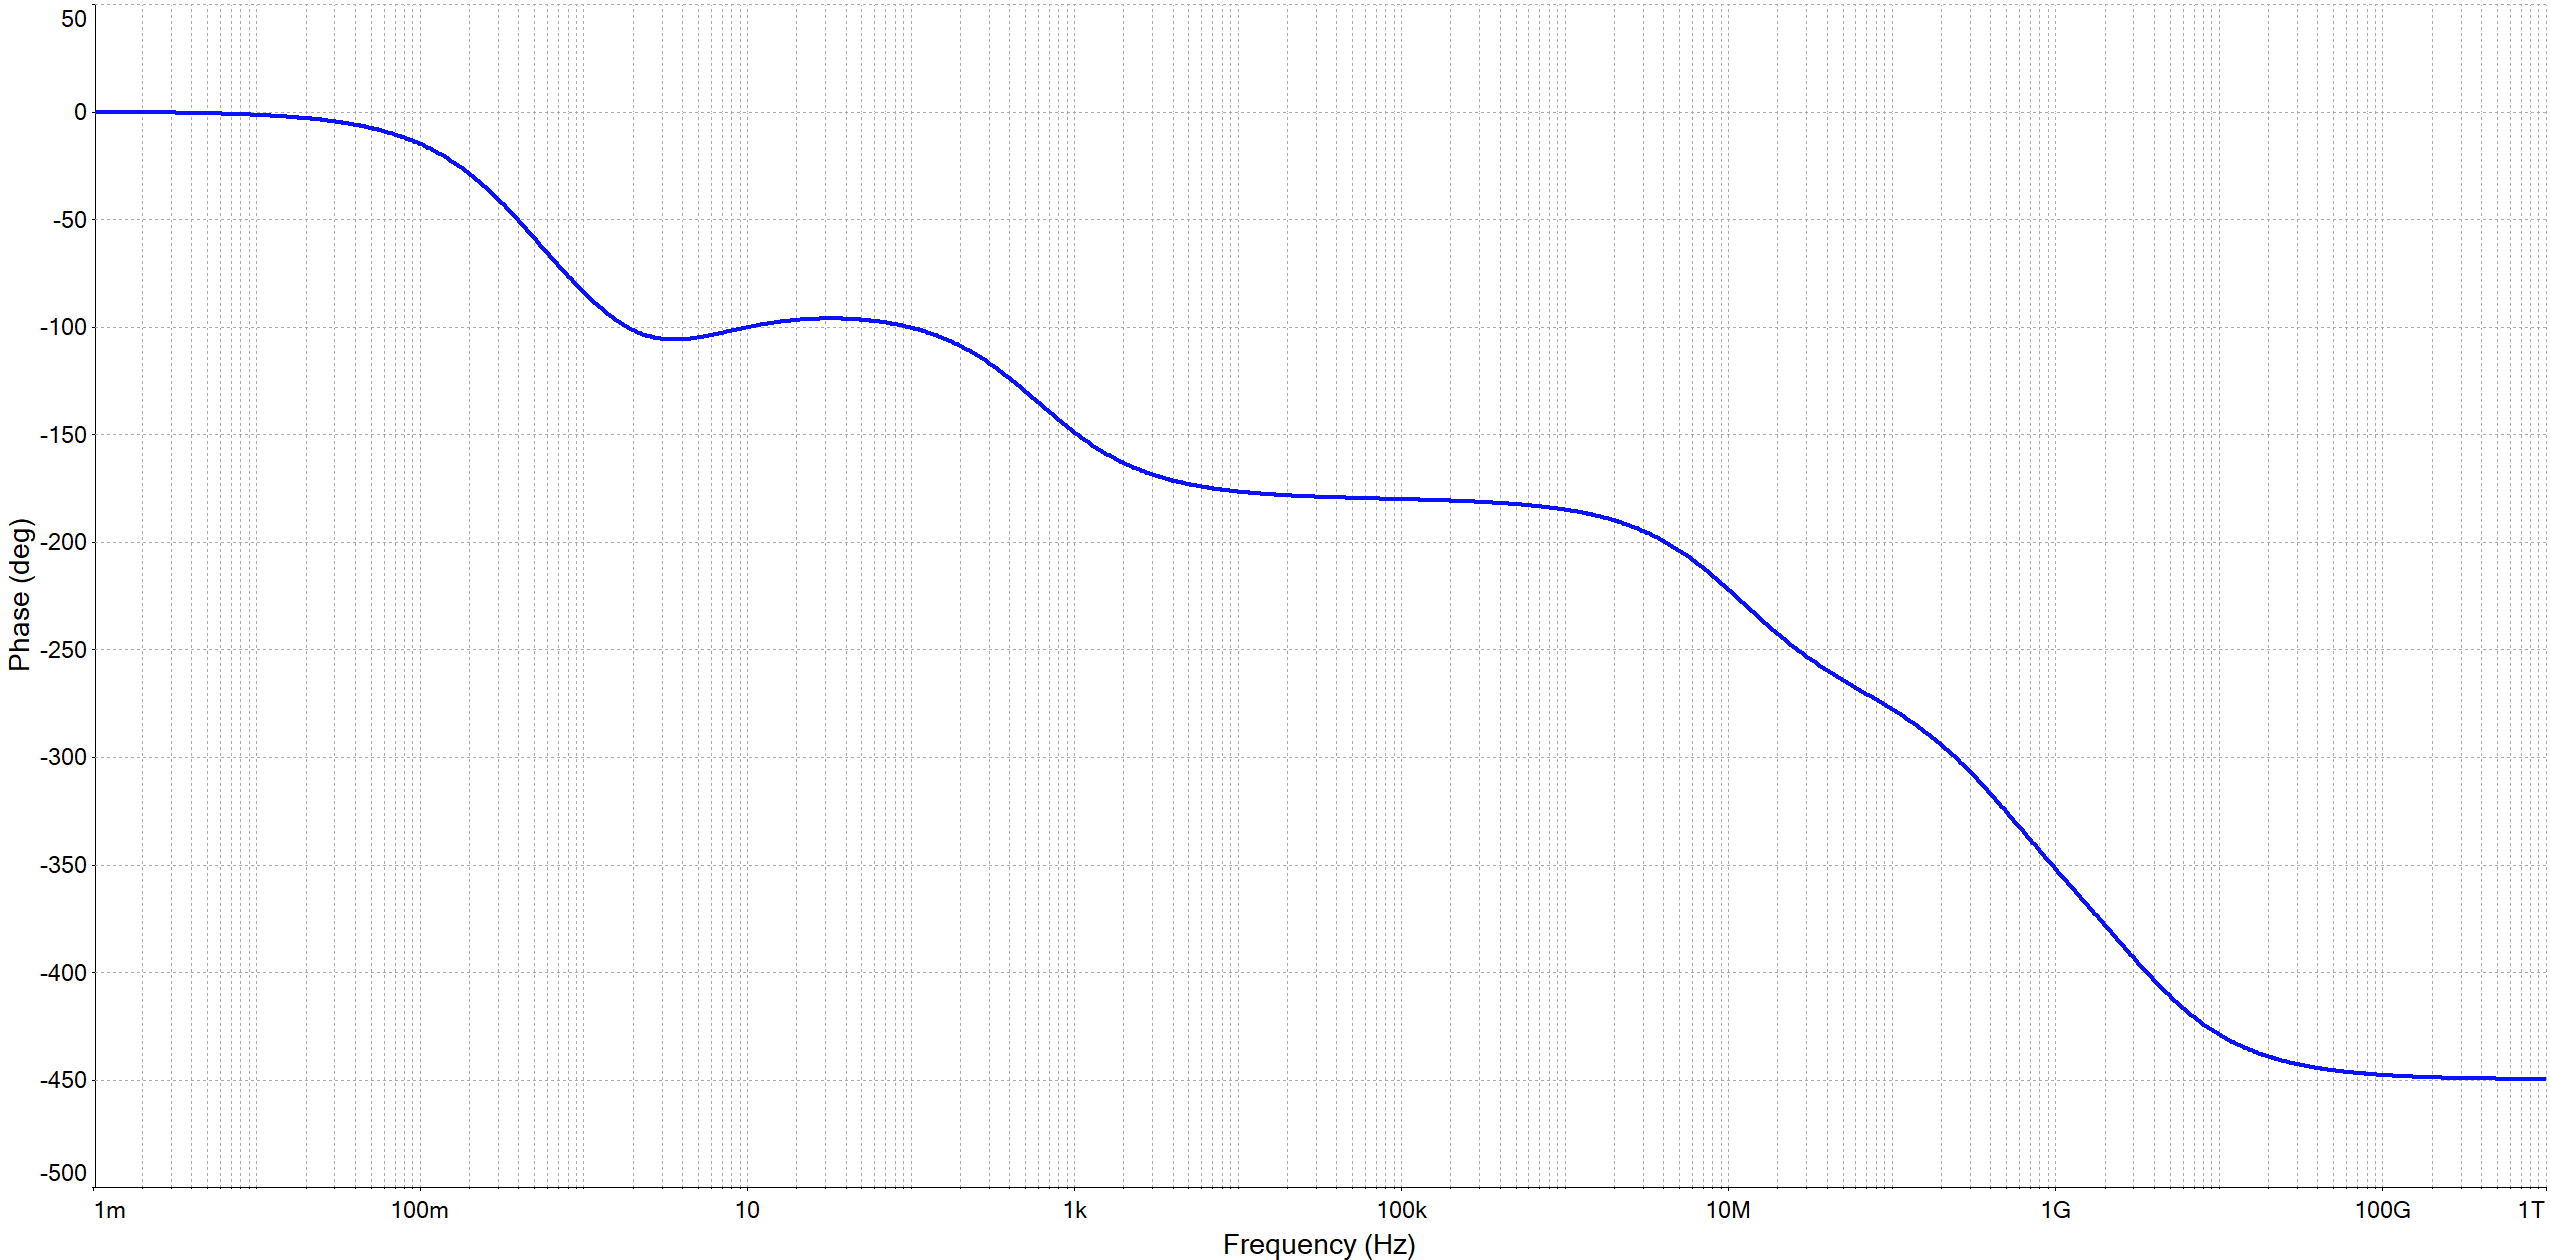
\includegraphics[height=0.45\textwidth]{Images/2a_2N3904_phase.png}\\
\caption{2N3904 Phase Plot}
\label{fig:part2a_phaseplot}
\end{figure}

Estimating the poles, we can see where the slope changes. From there, we can use the cursor in Multisim$^{TM}$ to find the pole frequencies. Here we can see the approximated poles and zeros from Figure \ref{fig:part2a_bodeplot_approximations} below:
\begin{figure}[H]
\centering
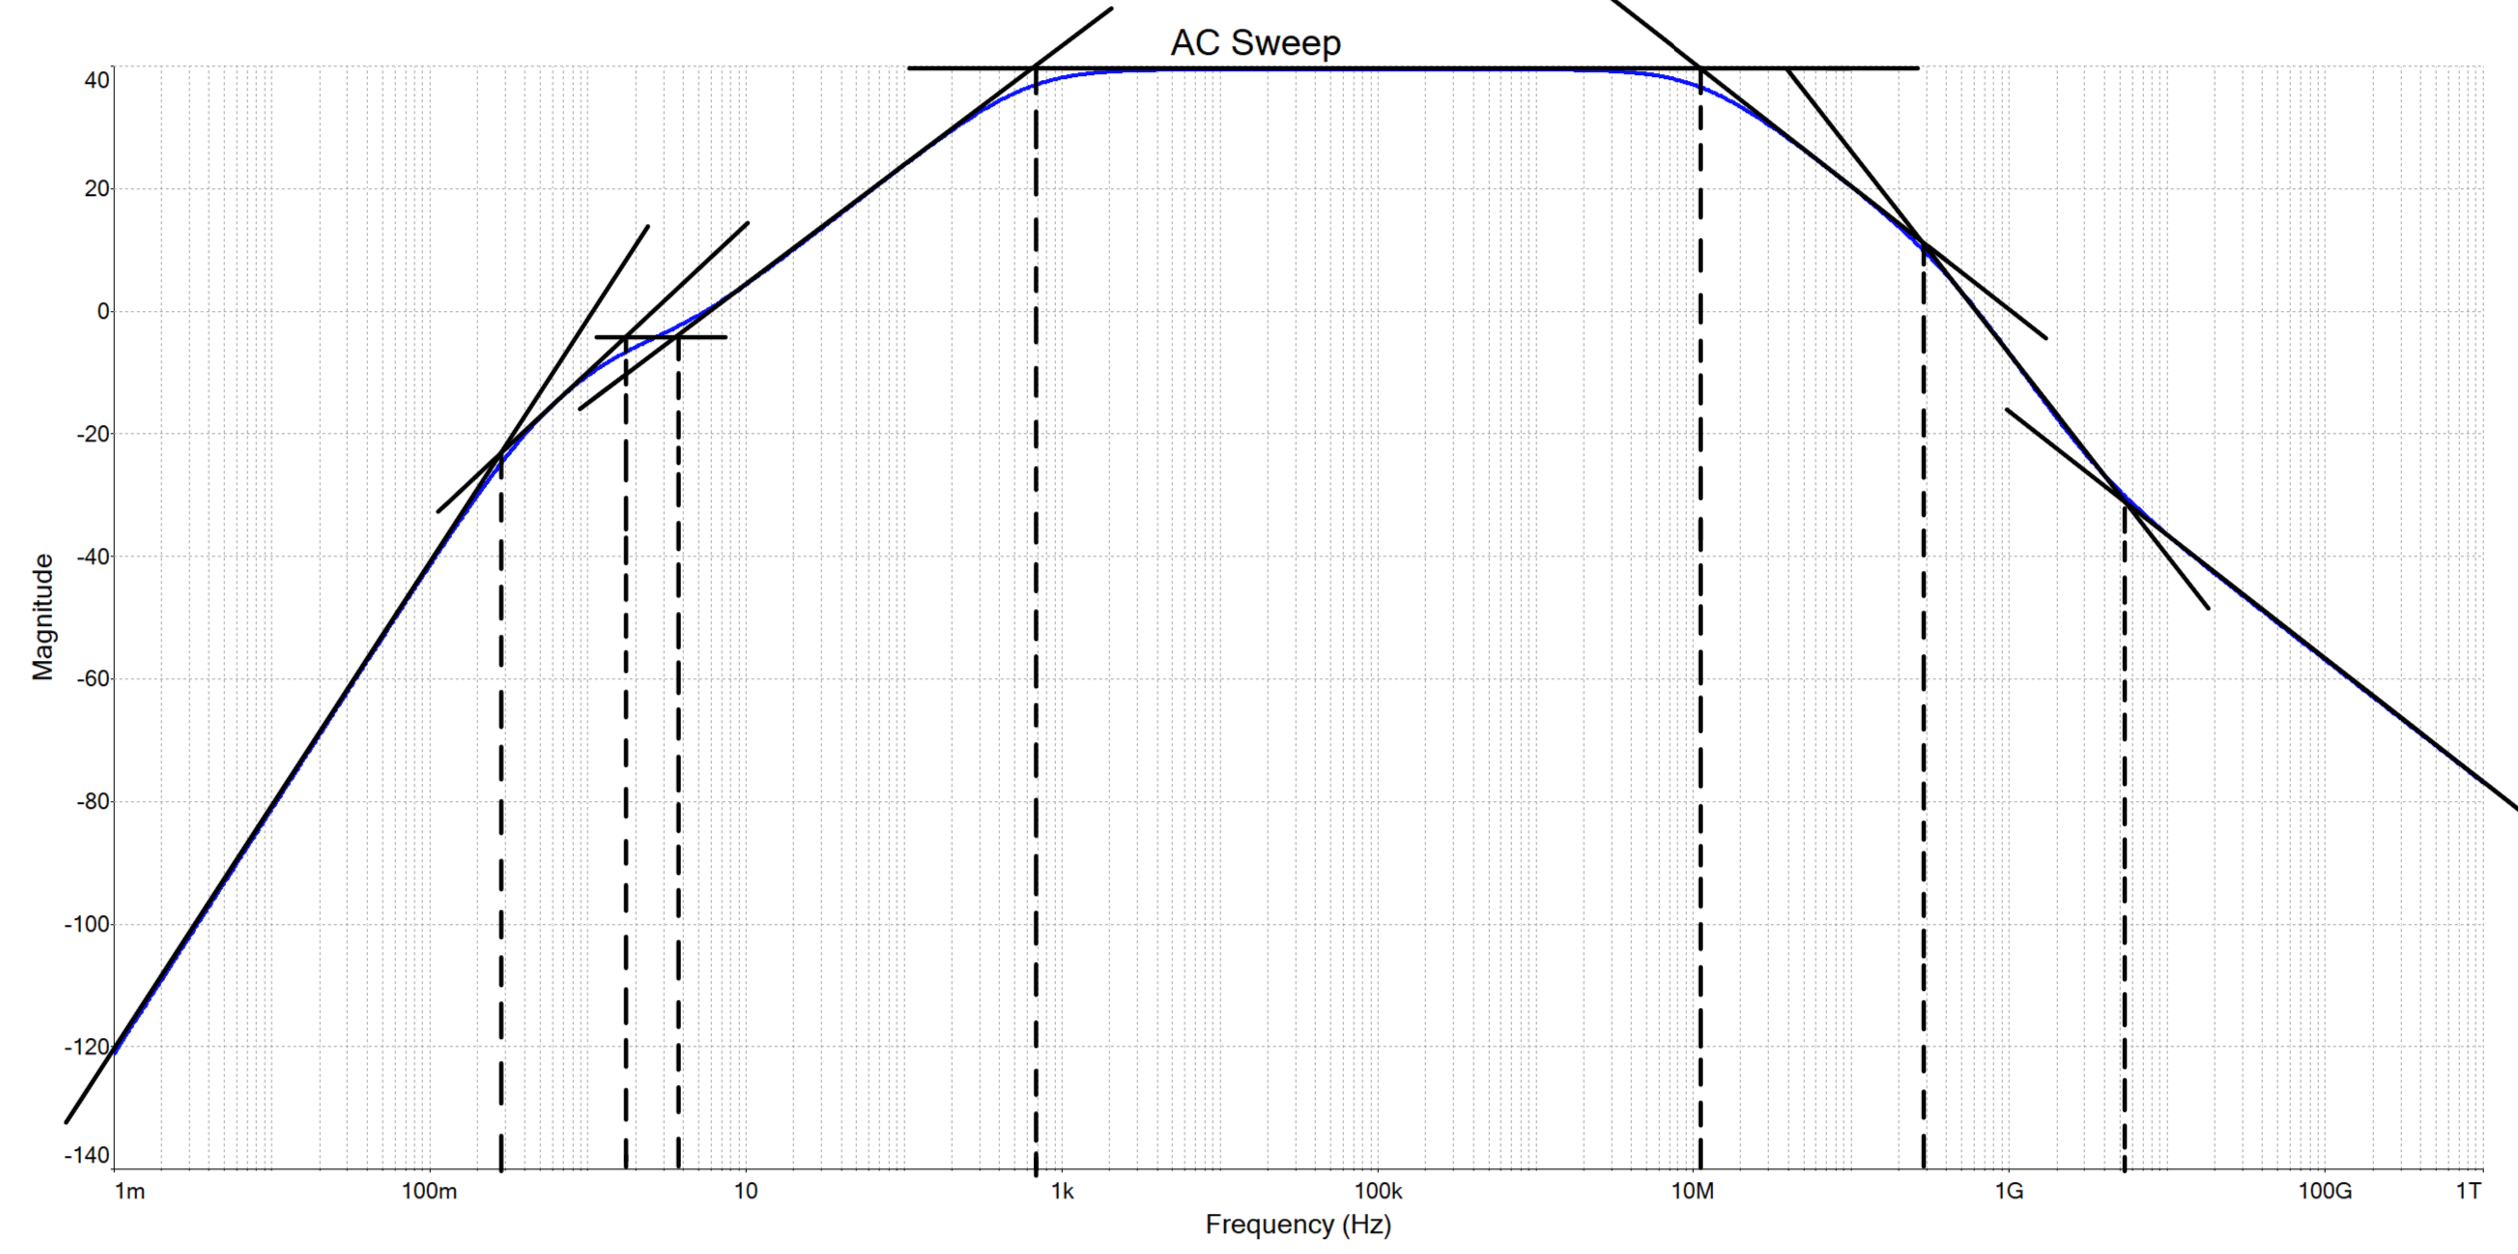
\includegraphics[height=0.45\textwidth]{Images/2abode_approximations.png}\\
\caption{2N3904 Bode Plot with Pole and Zero Approximations}
\label{fig:part2a_bodeplot_approximations}
\end{figure}

Here are the approximations:
\begin{table}[h!]
\centering
\begin{tabular}{|l|l|l|l|l|l|l|l|l|}
\cline{1-2} \cline{3-9}
             & $w_{lz1}$ & $w_{lz2}$ & $w_{lz3}$ & $w_{lp1}$  & $w_{lp2}$  & $w_{lp3}$     & $w_{hp1}$          & $w_{hp2}$           \\ \cline{1-2} \cline{3-9}
$w[\frac{rad}{s}]$ &  0    & 0     & 27.469      & 13.847 & 5.834 & 4005.283 & $94.231*10^6$ & $220.354*10^6$ \\
\hline
\end{tabular}
\caption{Table of Approximation of Pole Frequencies(2N3904)}
\label{table:2N3904_Approximation_Poles}
\end{table}

The calculations can be done with the equations as seen in class, which is no. 1. on the attached Appendix. 
Here are the calculations for the same transistor:
\begin{table}[h!]
\centering
\begin{tabular}{|l|l|l|l|l|l|l|l|l|}
\cline{1-2} \cline{3-9}
             & $w_{lz1}$ & $w_{lz2}$ & $w_{lz3}$ & $w_{lp1}$  & $w_{lp2}$  & $w_{lp3}$     & $w_{hp1}$          & $w_{hp2}$           \\ \cline{1-2} \cline{3-9}
$w[\frac{rad}{s}]$ &  0    & 0     & 23.256      & 9.804 & 2.713 & 3989.908 & $95.153*10^6$ & $215.996*10^6$ \\
\hline
\end{tabular}
\caption{Table of Calculated Pole Frequencies(2N3904)}
\label{table:2N3904_Calculated_Poles}
\end{table}

Comparing the calculated and approximated pole frequencies, we can conclude that the low frequency estimates are relatively accurate. Furthermore, we can also conclude that the high frequency estimates are accurate as well.

%----------------------2N4401 Transistor--------------------------------

Here is the bode and phase plot for a Common Emitter Amplifier with the 2N4401 Transistor:

\begin{figure}[H]
\centering
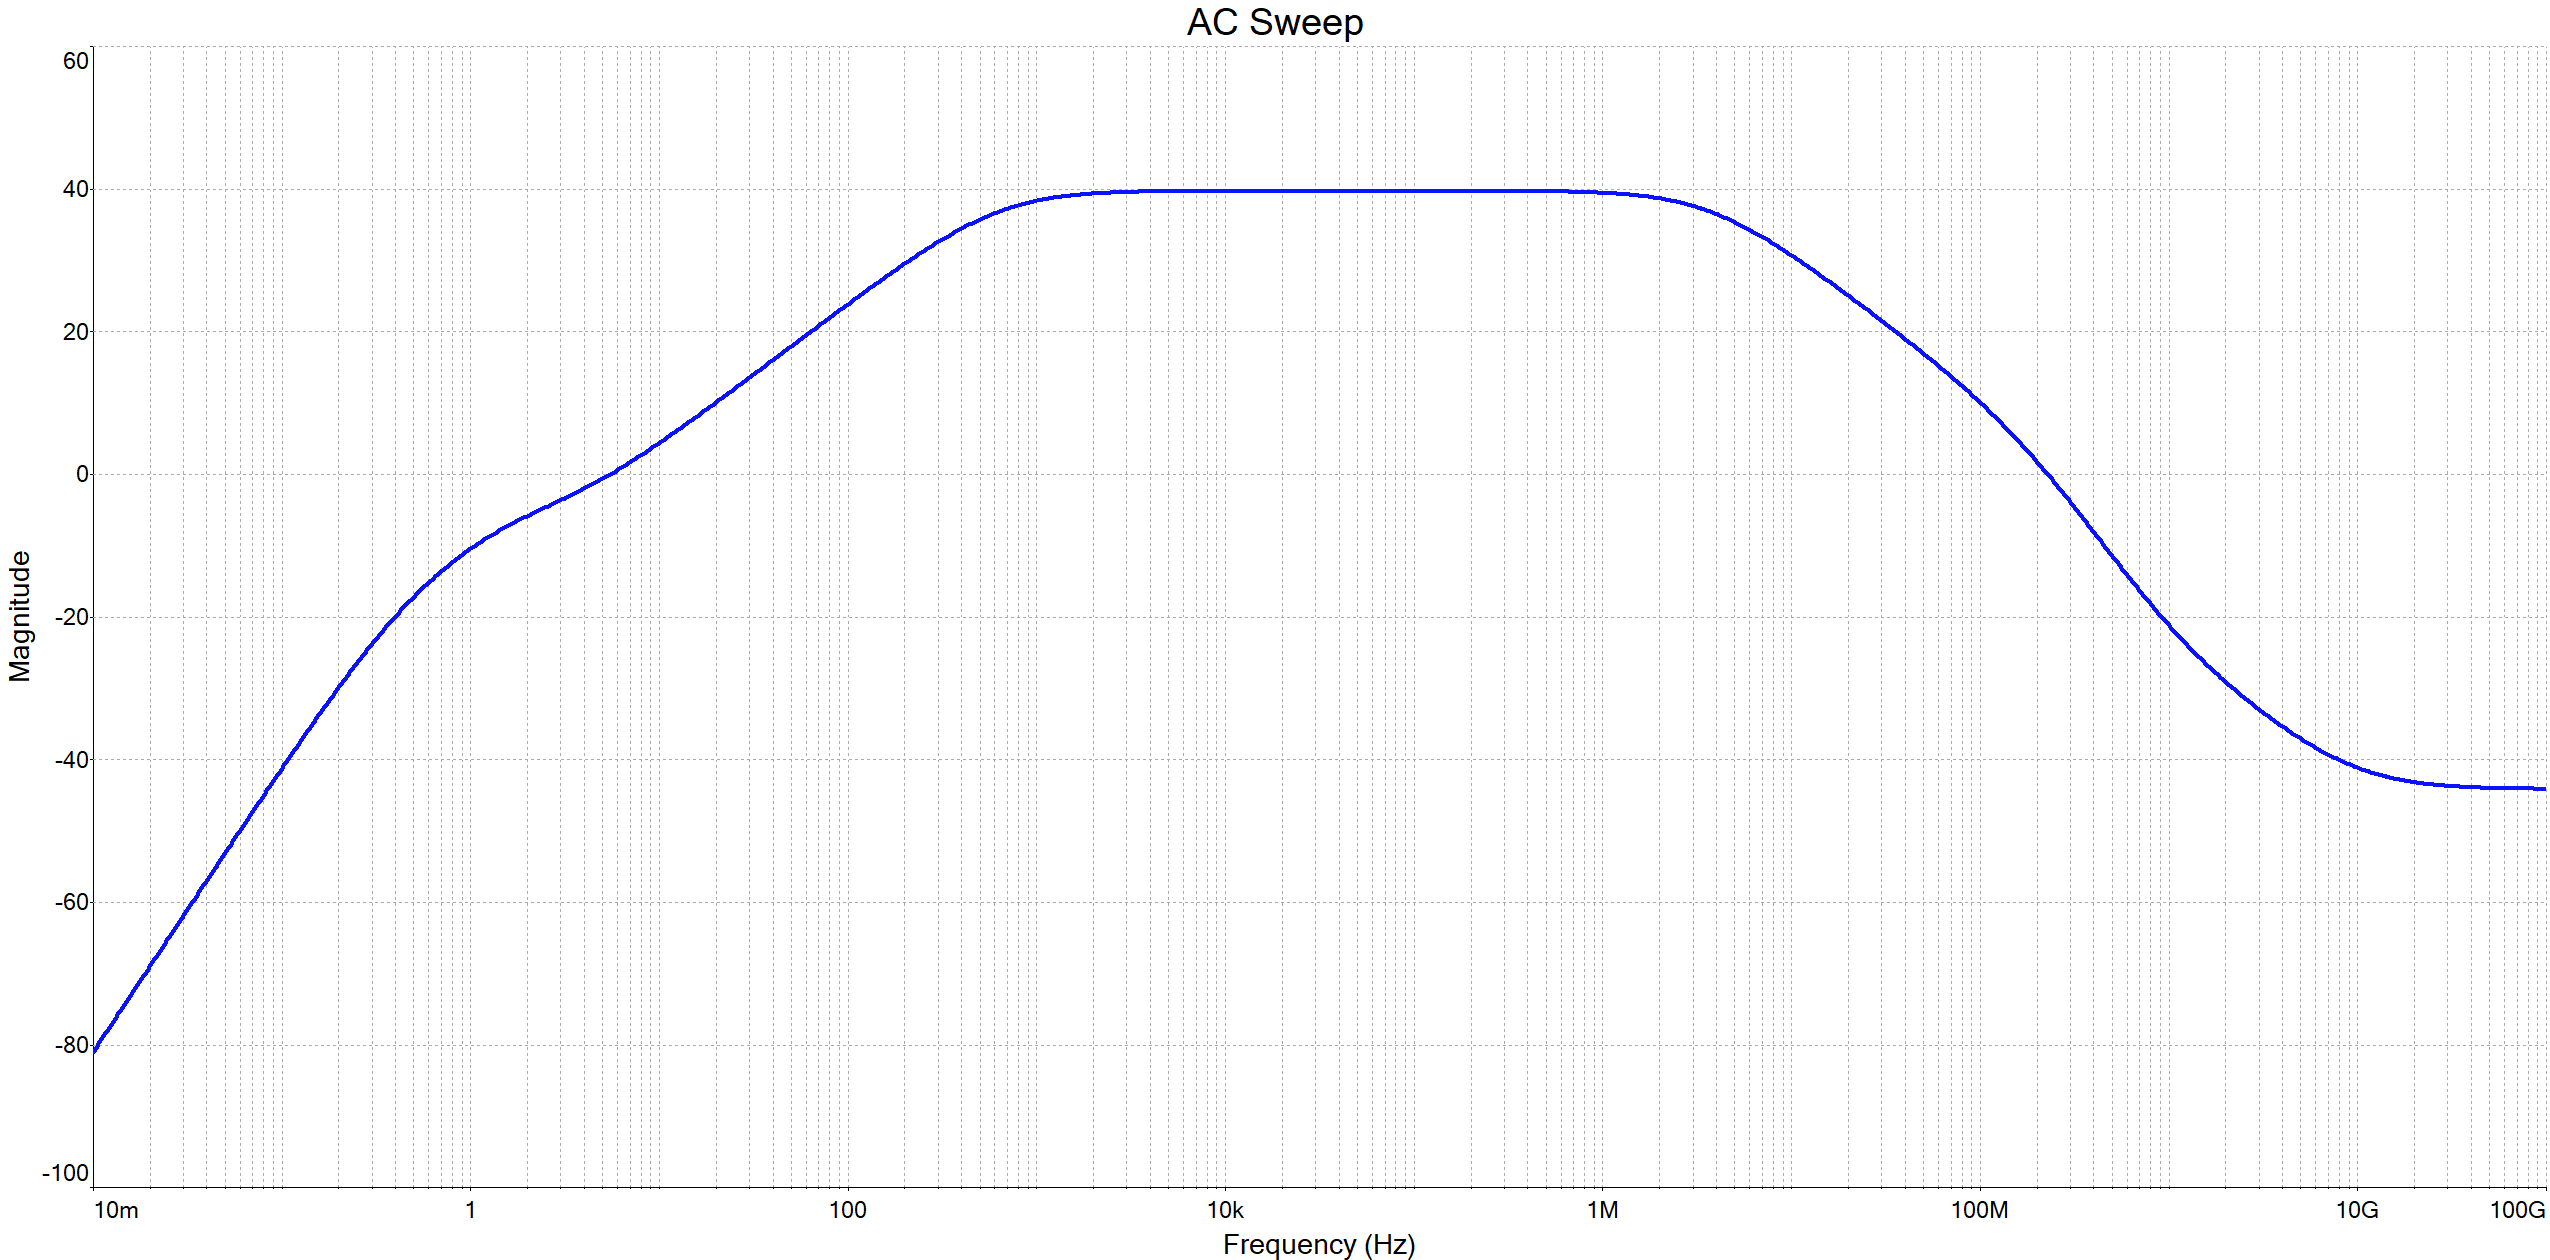
\includegraphics[height=0.45\textwidth]{Images/2a_2N4401}\\
\caption{2N4401 Bode Plot}
\label{fig:part2a_bodeplot_2N4401}
\end{figure}

\begin{figure}[H]
\centering
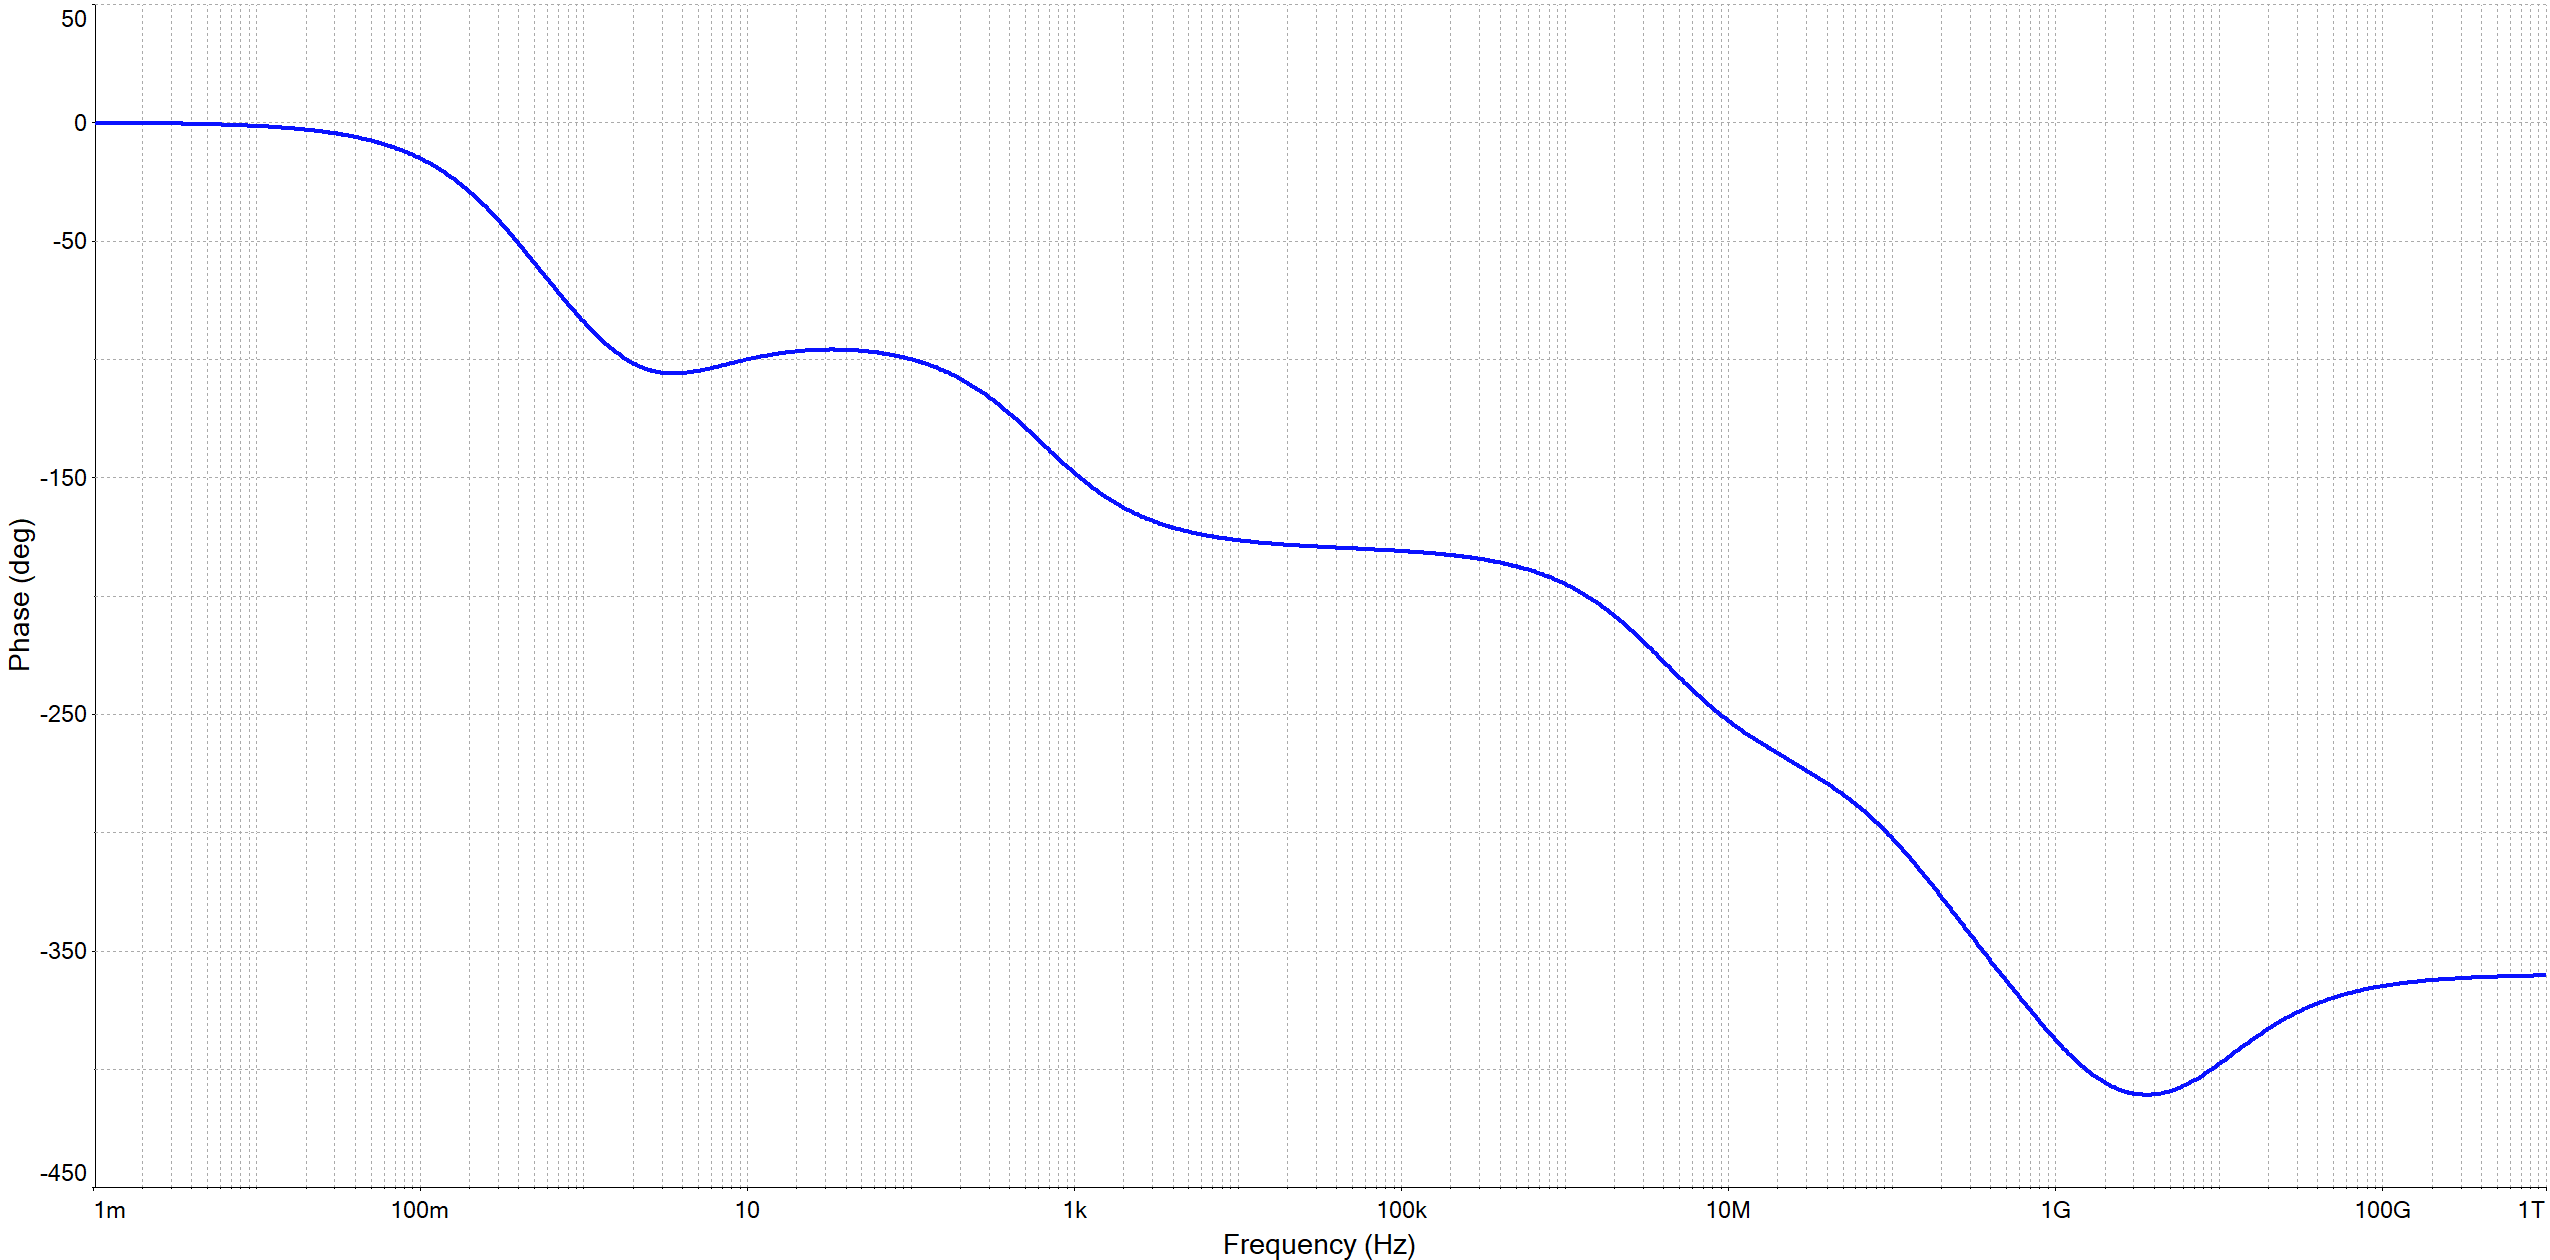
\includegraphics[height=0.45\textwidth]{Images/2a_2N4401_phase.png}\\
\caption{2N4401 Phase Plot}
\label{fig:part2a_phase_plot_2N4401}
\end{figure}

Here are the zero and pole approximations:

\begin{figure}[H]
\centering
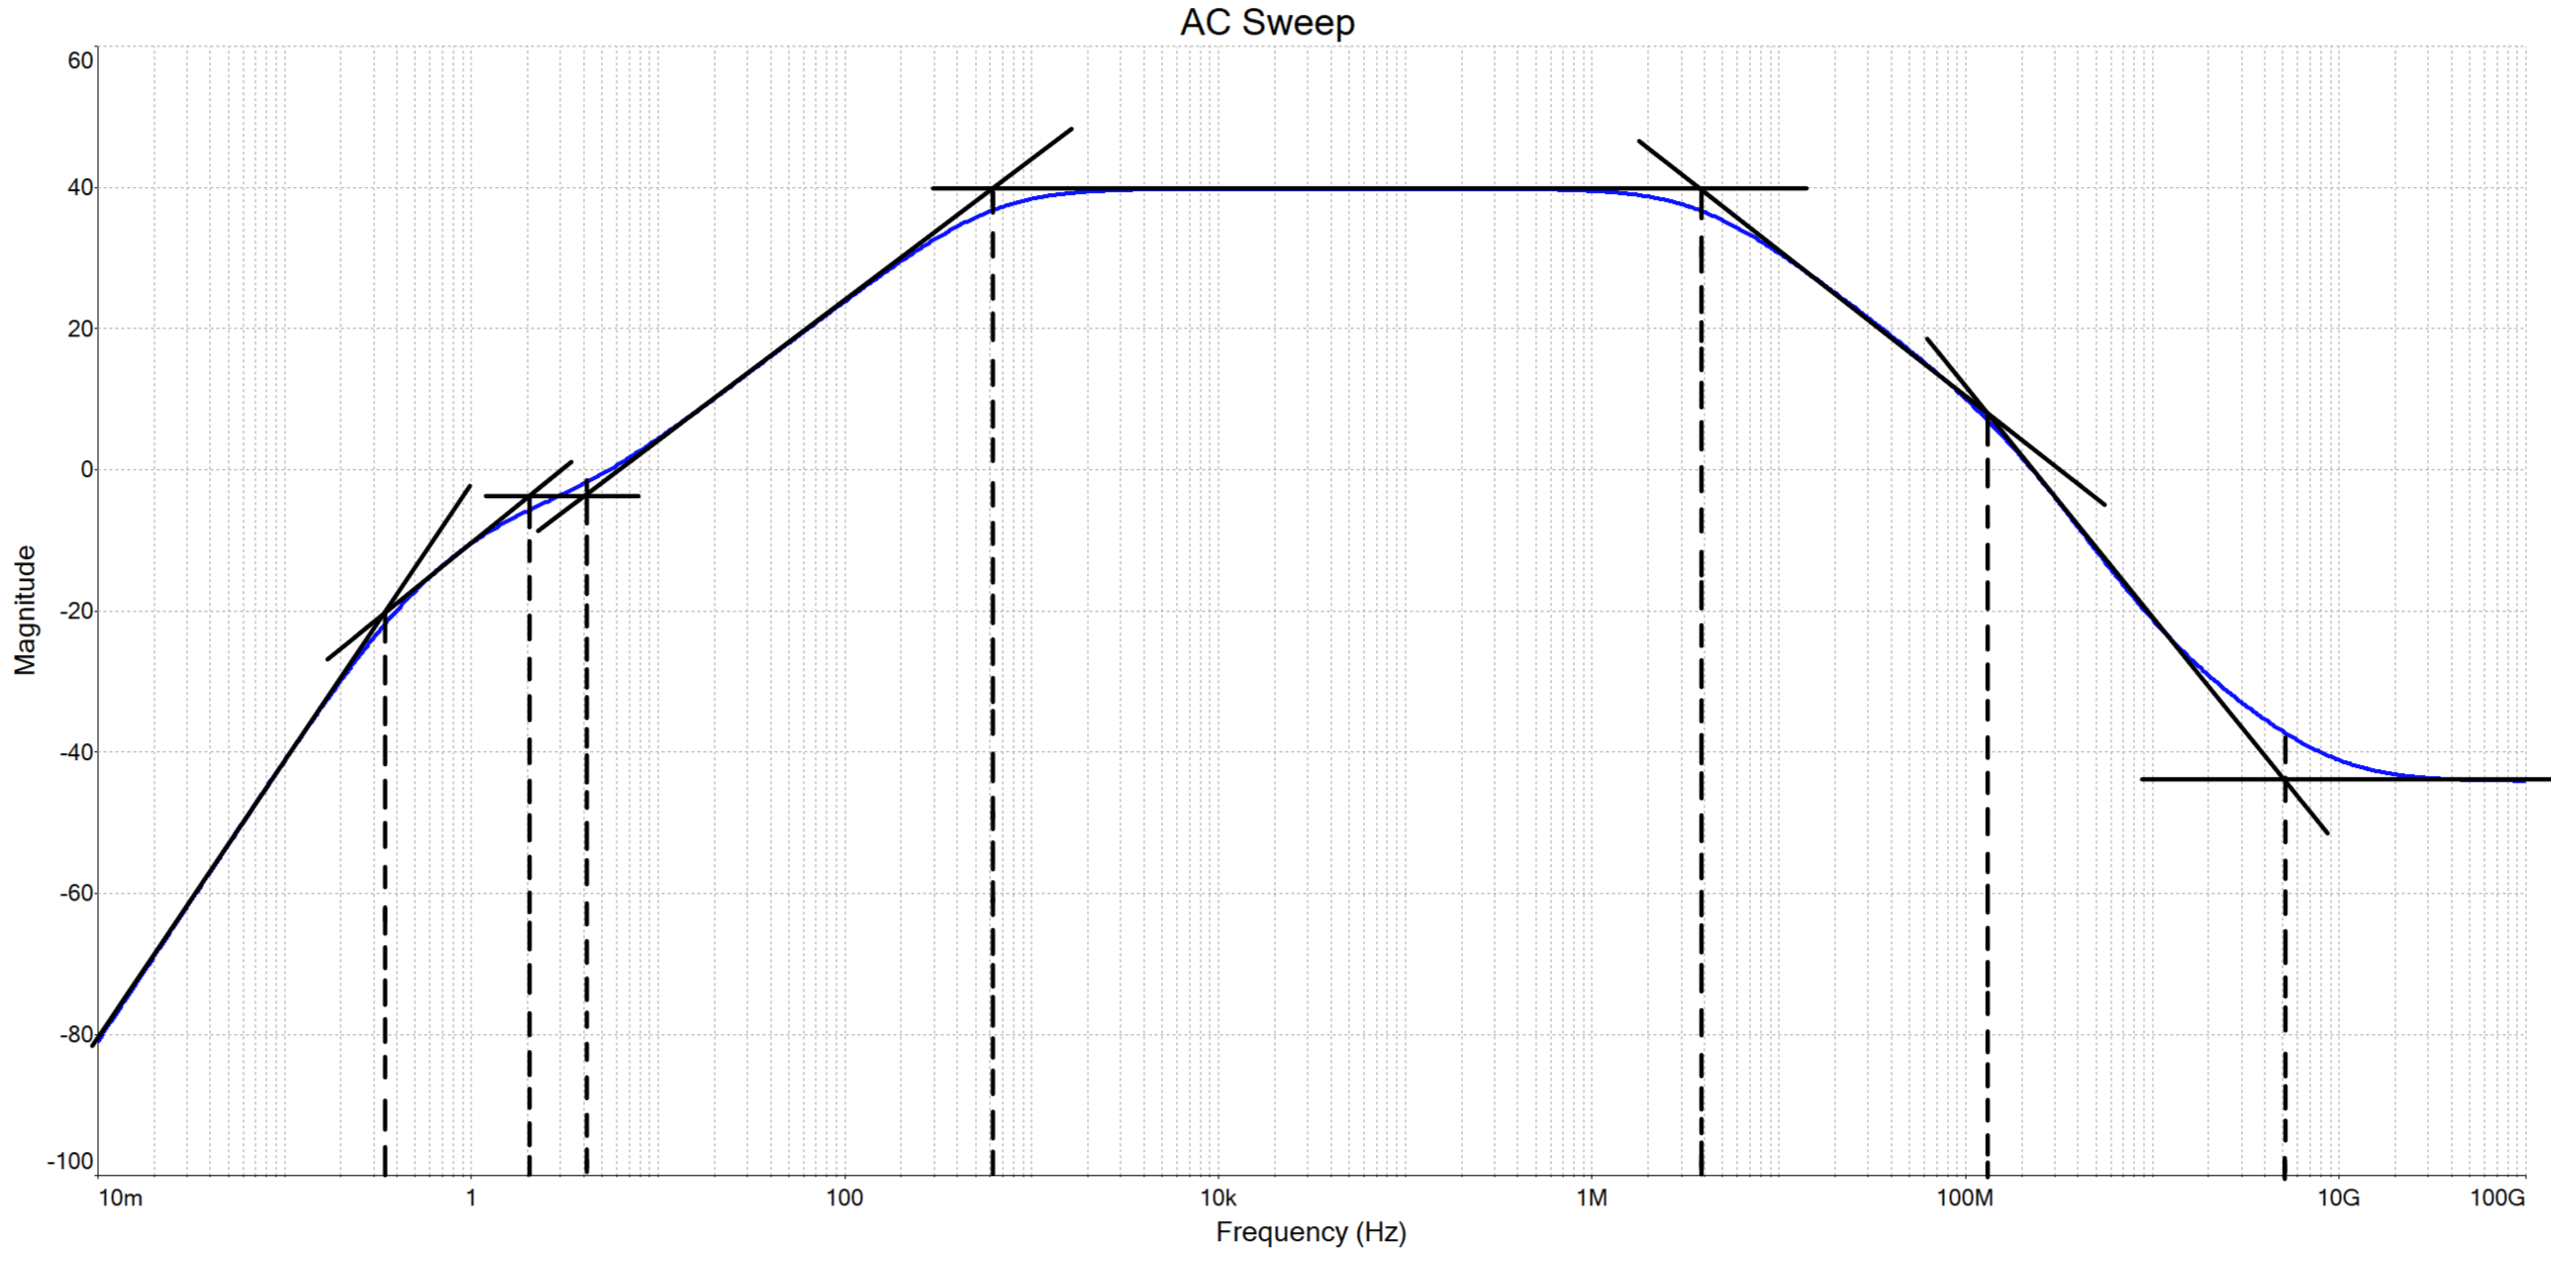
\includegraphics[height=0.45\textwidth]{Images/2abode_approximations_2N4401.png}\\
\caption{2N4401 Bode Plot with zero and pole approximations}
\label{fig:part2a_bodeplot_approximations_2N4401}
\end{figure}

Doing the same approximations as the previous transistor, we can see that the approximations for the pole frequencies are:
\begin{table}[h!]
\centering
\begin{tabular}{|l|l|l|l|l|l|l|l|l|}
\cline{1-2} \cline{3-9}
             & $w_{lz1}$ & $w_{lz2}$ & $w_{lz3}$ & $w_{lp1}$  & $w_{lp2}$  & $w_{lp3}$     & $w_{hp1}$          & $w_{hp2}$           \\ \cline{1-2} \cline{3-9}
$w[\frac{rad}{s}]$ &  0    & 0     & 25.572      & 10.365 & 2.772 & 4103.805 & $33.954*10^6$ & $80.079*10^6$ \\
\hline
\end{tabular}
\caption{Table of Approximation of Pole Frequencies(2N4401)}
\label{table:2N4401_Approximation_Poles}
\end{table}

We can also do the same calculation as shown in no. 1 in the Appendix to find the pole frequencies for this transistor, and the calculated values are:

\begin{table}[h!]
\centering
\begin{tabular}{|l|l|l|l|l|l|l|l|l|}
\cline{1-2} \cline{3-9}
             & $w_{lz1}$ & $w_{lz2}$ & $w_{lz3}$ & $w_{lp1}$  & $w_{lp2}$  & $w_{lp3}$     & $w_{hp1}$          & $w_{hp2}$           \\ \cline{1-2} \cline{3-9}
$w[\frac{rad}{s}]$ &  0    & 0     & 23.256      & 9.804 & 2.677 & 4048.325 & $32.320*10^6$ & $73.527*10^6$ \\
\hline
\end{tabular}
\caption{Table of Calculated Pole Frequencies(2N4401)}
\label{table:2N3904_Calculated_Poles}
\end{table}

Here we can conclude that the calculations and the approximations are relatively accurate.
\subsubsection{Part b)}

For the midband frequency, we can choose that it will be 100kHz. Varying the input voltage from 0-0.1V and plotting $\frac{v_o}{v_s}$:

\begin{figure}[H]
\centering
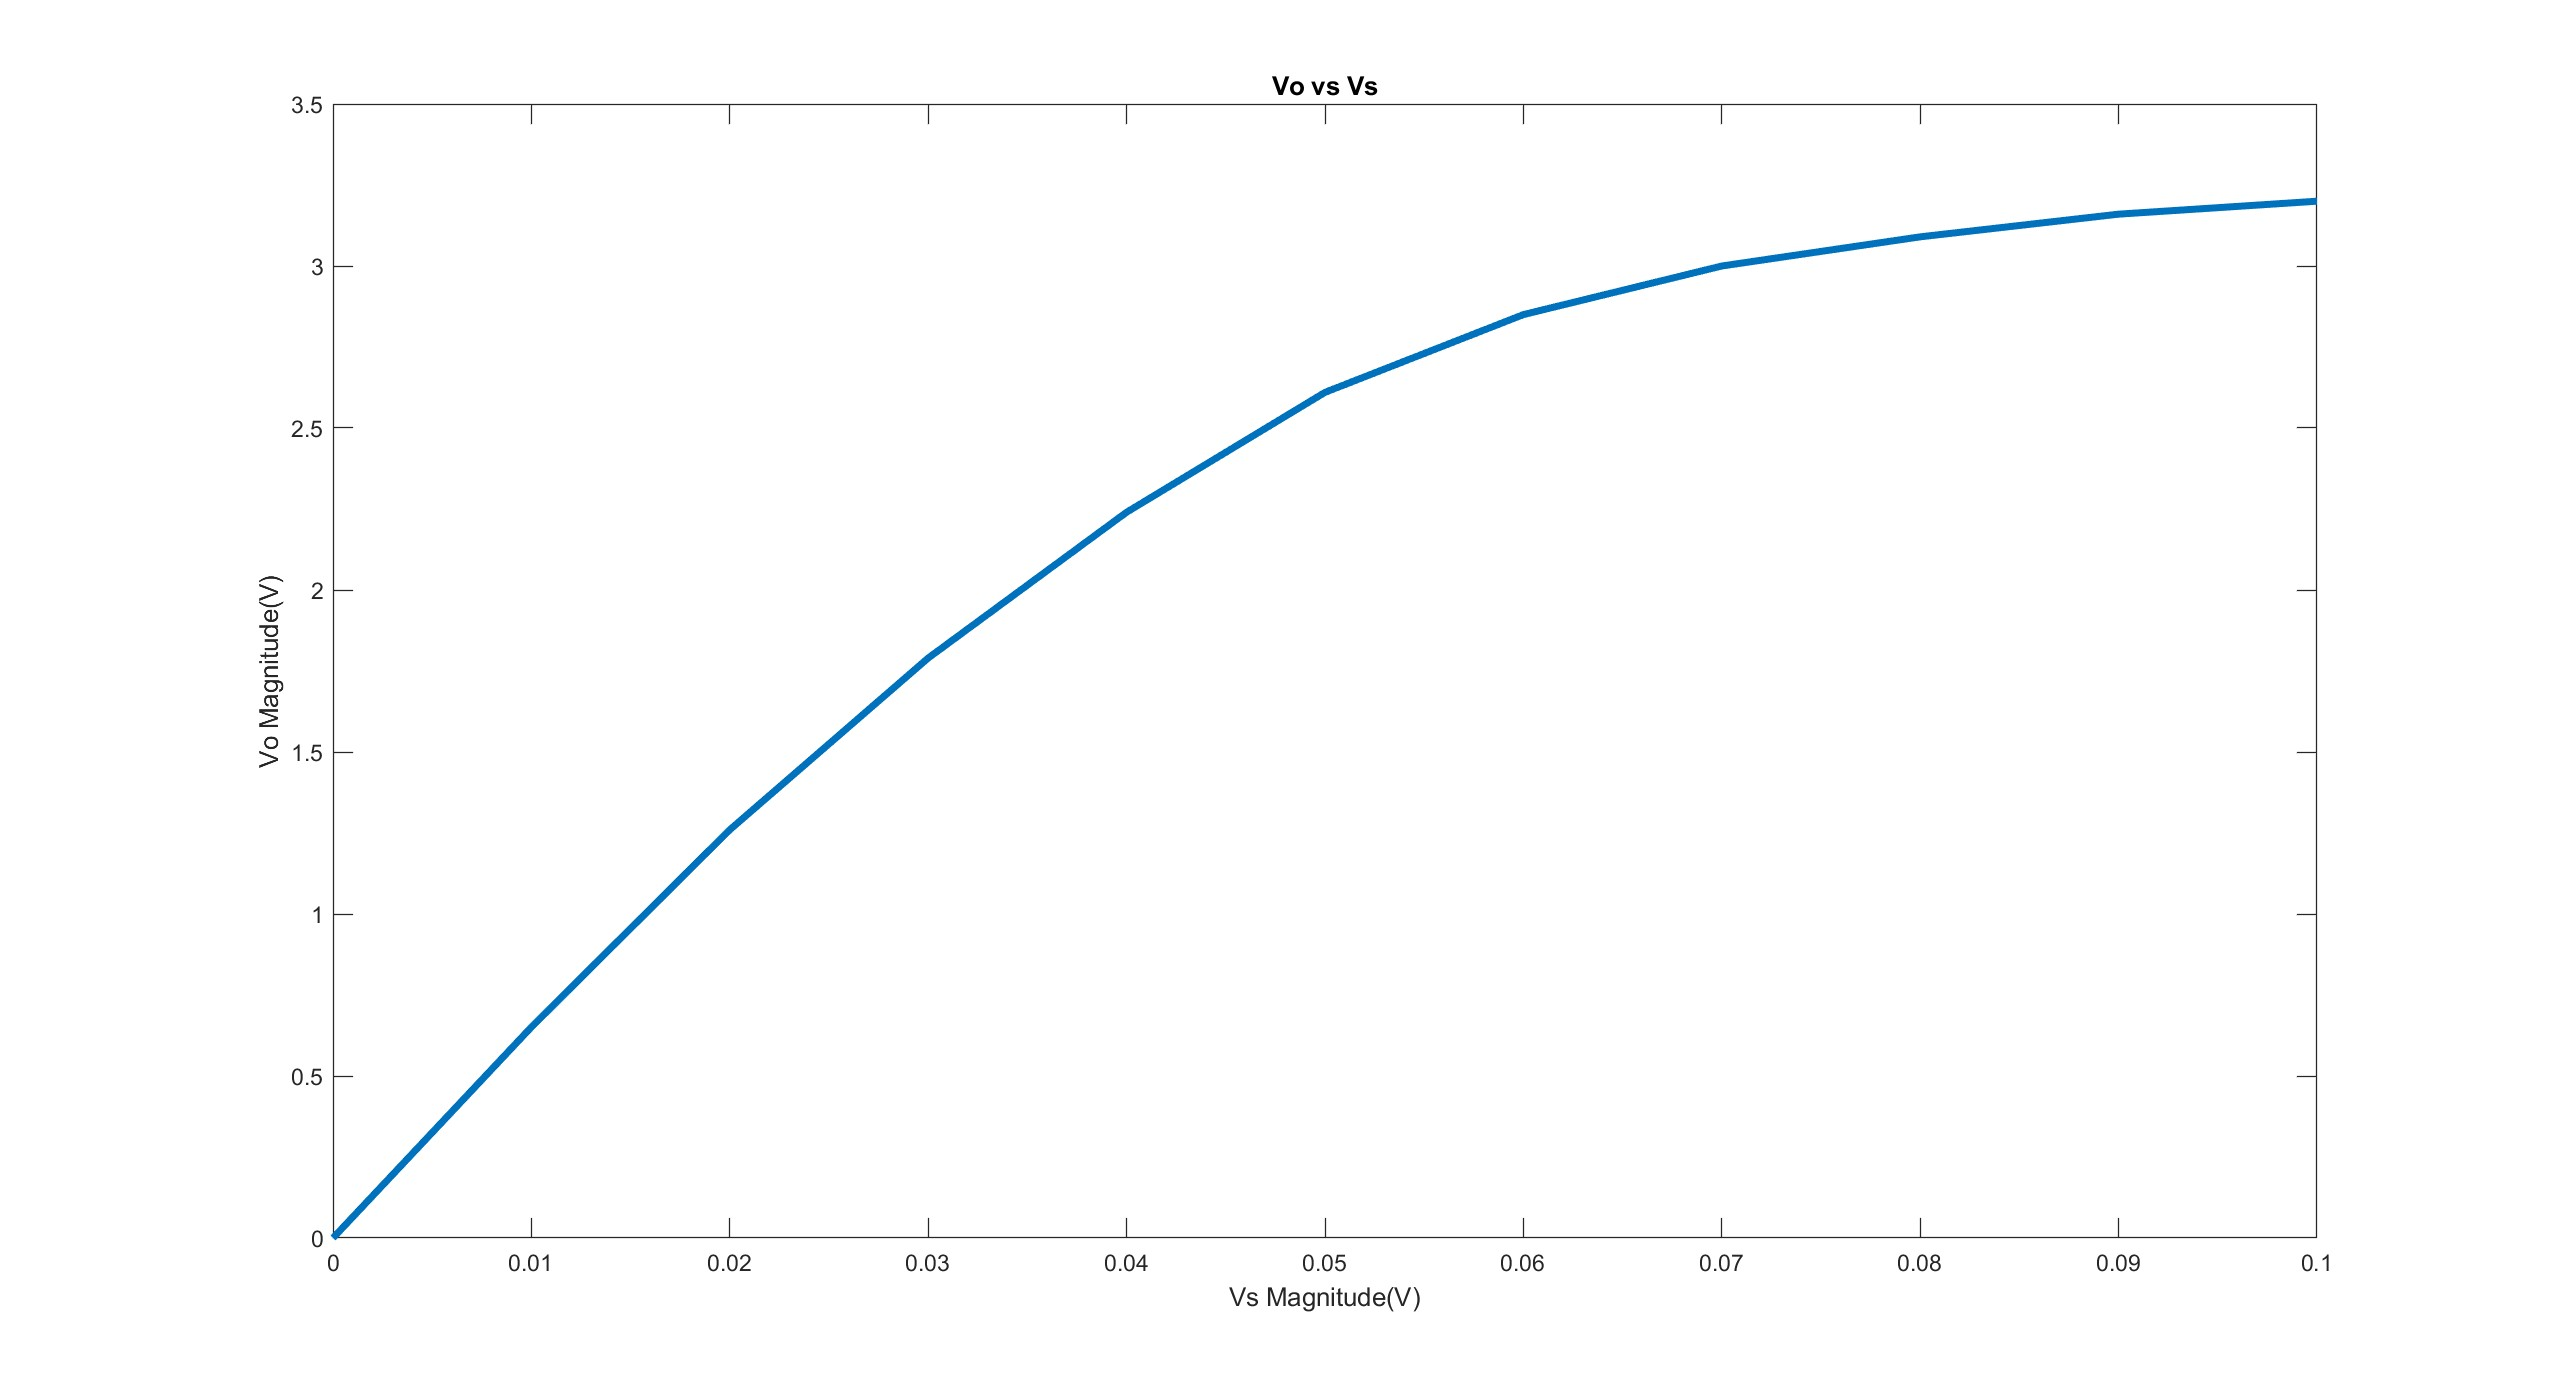
\includegraphics[height=0.45\textwidth]{Images/voltage_transfer_plot.jpg}\\
\caption{$V_o$ vs $V_s$(2N3904)}
\label{fig:transfer_plot_2N3904}
\end{figure}
Here is the voltage transfer plot for the 2N4401 Transistor:
\begin{figure}[H]
\centering
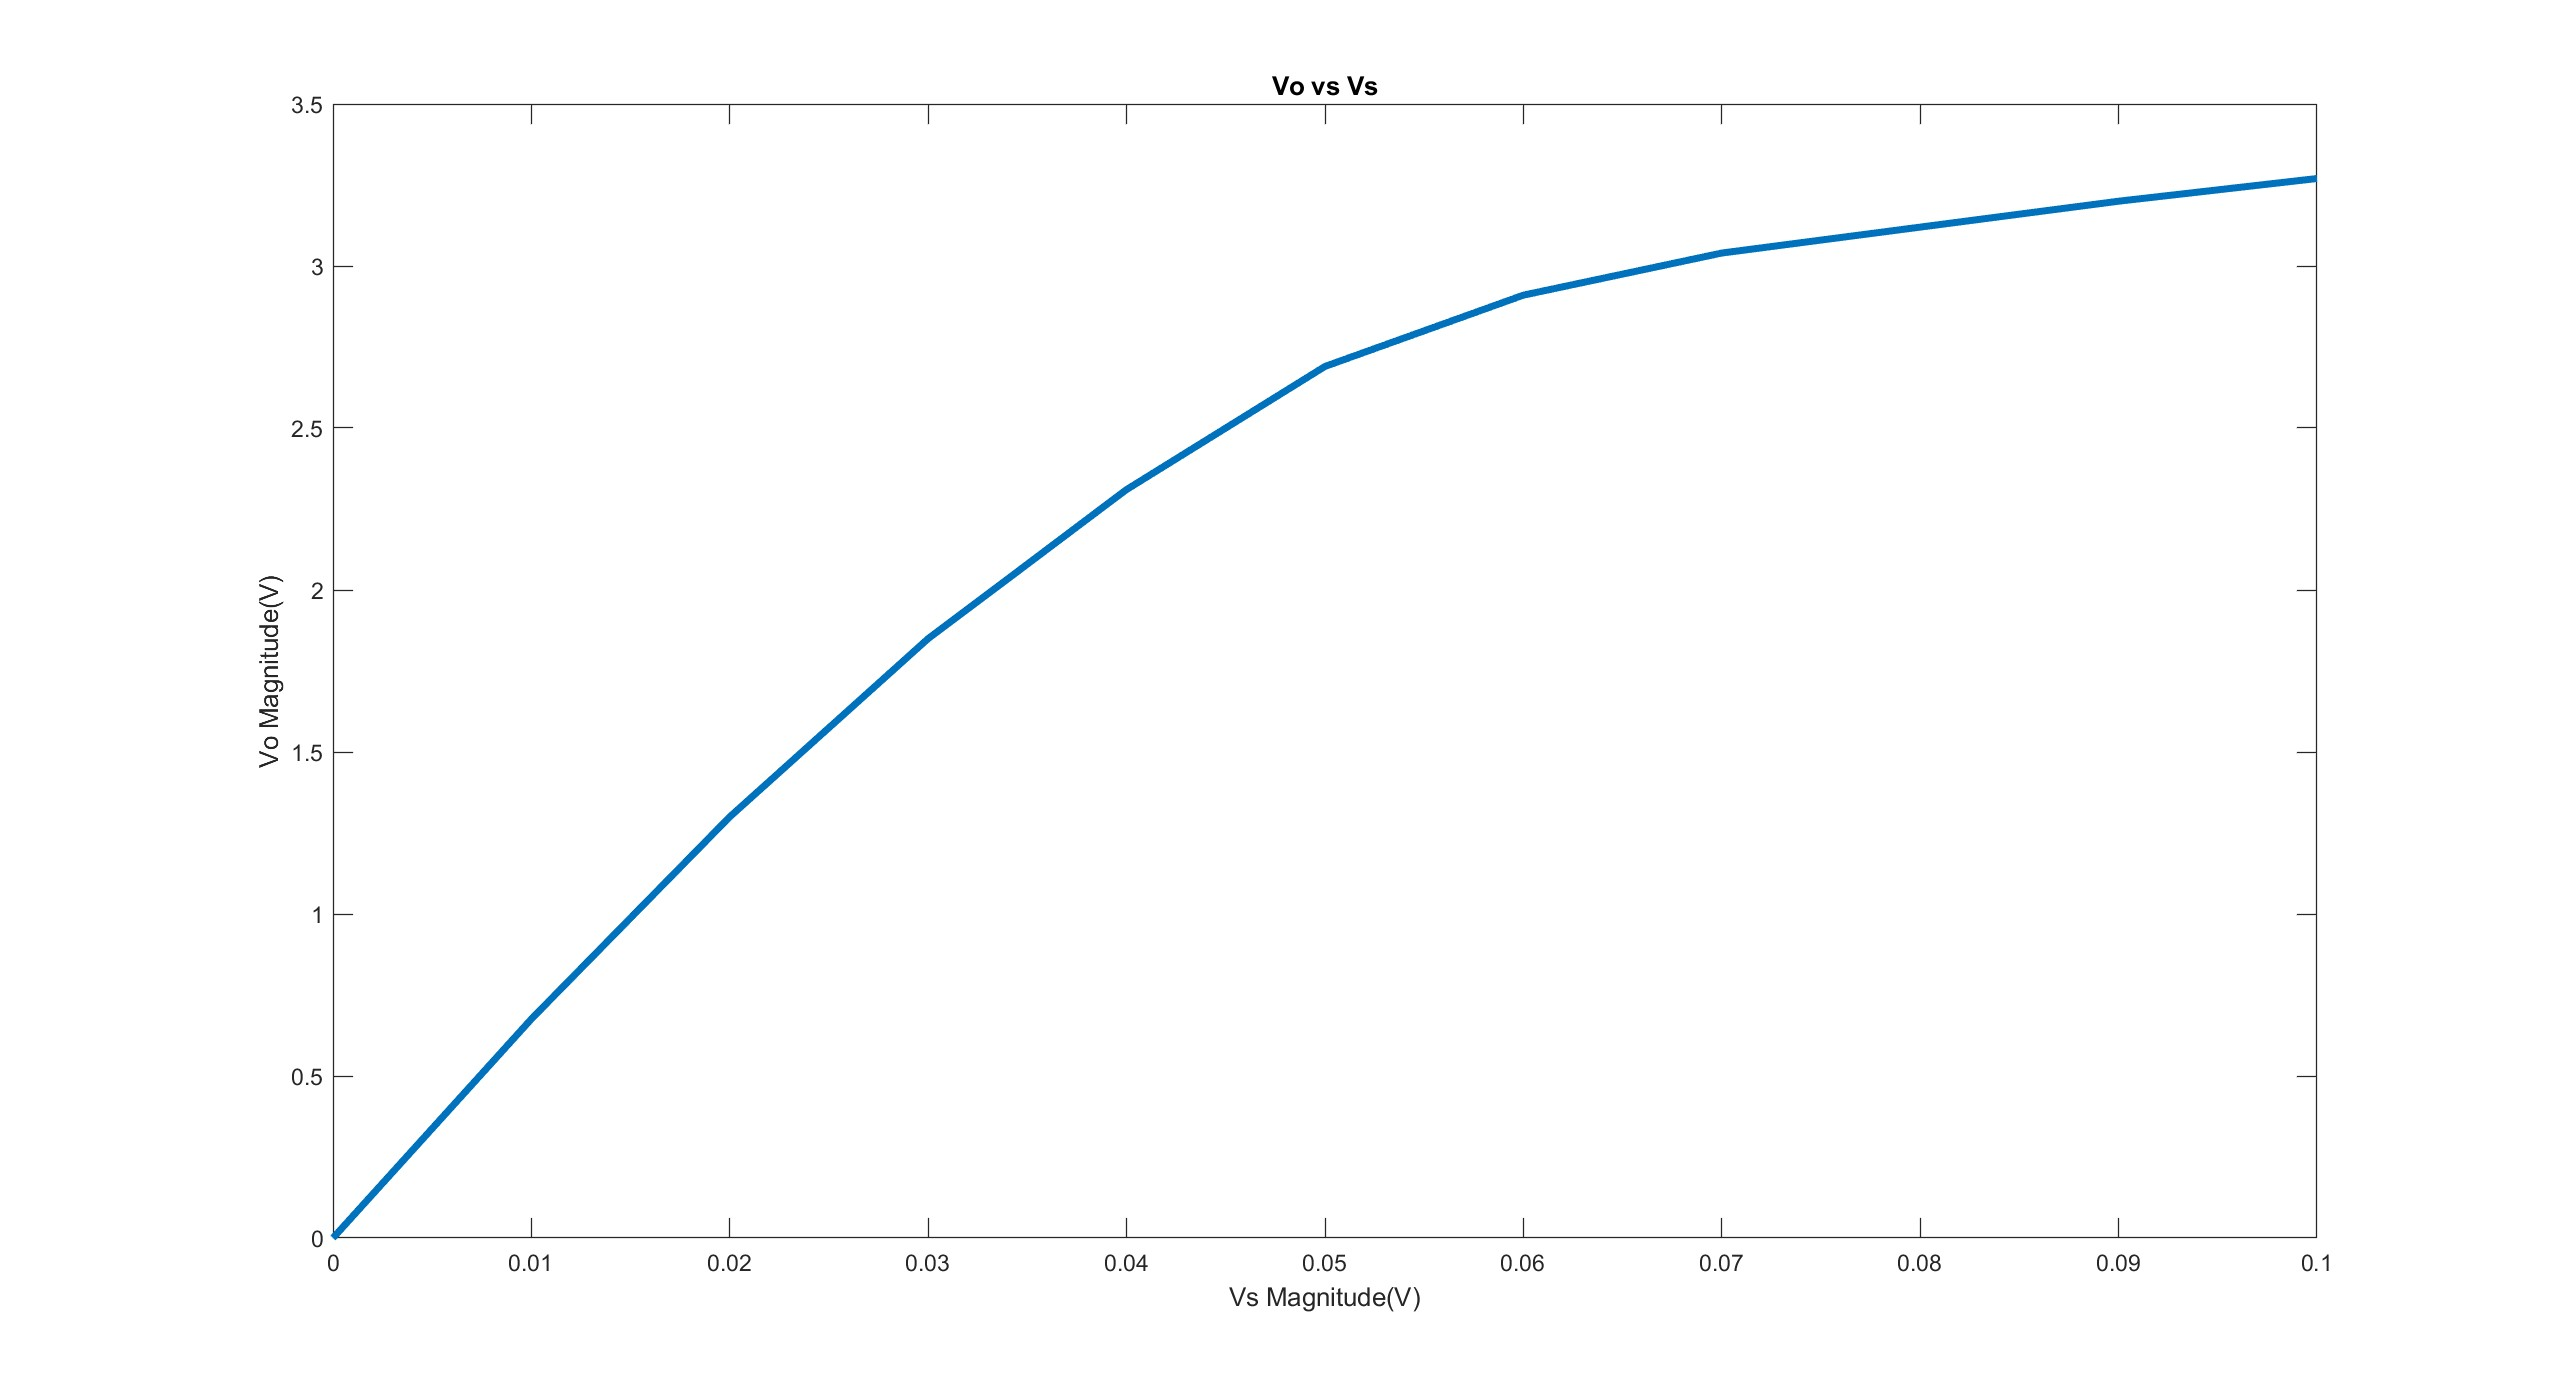
\includegraphics[height=0.45\textwidth]{Images/voltage_transfer_plot_2N4401.jpg}\\
\caption{$V_o$ vs $V_s$(2N4401)}
\label{fig:transfer_plot_2N3904}
\end{figure}

Here we can see that the plots of each transfer function is not linear when the input voltage is 0.03V at midband frequency for the 2N3904. For the 2N4401, we can see it is not linear around 0.04V. 

\subsubsection{Part c) and d)}


To measure the input impedance for the 2N3904, we can use the multimeter in Multisim$^{TM}$. We can find the current in the input/output and the voltage in the input/output. We will also be setting the frequency of our power supply at 100kHz (mid-band frequency) and our voltage amplitude to be 0.01V. For the input, we will measure the current going across $C_{C1}$ and we can also measure the voltage at $C_{C1}$ as well. To find the impedance for the output, we will measure the current going across the load resistor, and the voltage across it as well.  Using this method, we find:
\begin{center}
$R_{in}=\frac{6.96mV}{2.222\mu A}$ = \boxed{3.132k\Omega}, $R_{out}=\frac{651mV}{128u A}$ = \boxed{5.086k\Omega}
\end{center}
To calculate the input and output impedance, we can use the formulas in no. 2 in the Appendix. We find that the values are:
\begin{center}
$R_{in}$= \boxed{2.738k\Omega}, $R_{out}$=\boxed{5.1k\Omega}    
\end{center}

For the 2N4401, we find that the measured values are:
\begin{center}
$R_{in}=\frac{6.99mV}{3.02\mu A}$ = \boxed{2.314k\Omega}, $R_{out}=\frac{676mV}{133\mu A}$ = \boxed{5.083k\Omega}
\end{center}
And the calculated values are:
\begin{center}
$R_{in}$= \boxed{3.29k\Omega}, $R_{out}$=\boxed{5.1k\Omega}
\end{center}

\subsubsection{Part e)}
Concluding from the results of the previous part, we can observe that the calculated values of the input resistance of the 2N4401 transistor does not match very well with it's corresponding measured values. However the calculated output resistance matches very well with it's measured output resistance. For the 2N3904, it can be observed that the measured input and output resistance matches closely to the calculated values. We can also see from the voltage transfer curve where the curve starts to become non-linear. The 2N4401 starts to become non-linear at a higher voltage than the 2N3904. However, the 2N3904 has a much larger bandwidth. Comparing the two transistors, the 2N3904 has better overall performance, since the 2N4401 does not become saturated for much longer than the 2N3904.
\section{Part 3}
\subsubsection{Part a)}
Here is the Common Base amplifier circuit with the 2N2222A transistor (named CM2N2222A since this is an imported SPICE model) that we will be analyzing:
\begin{figure}[H]
\centering
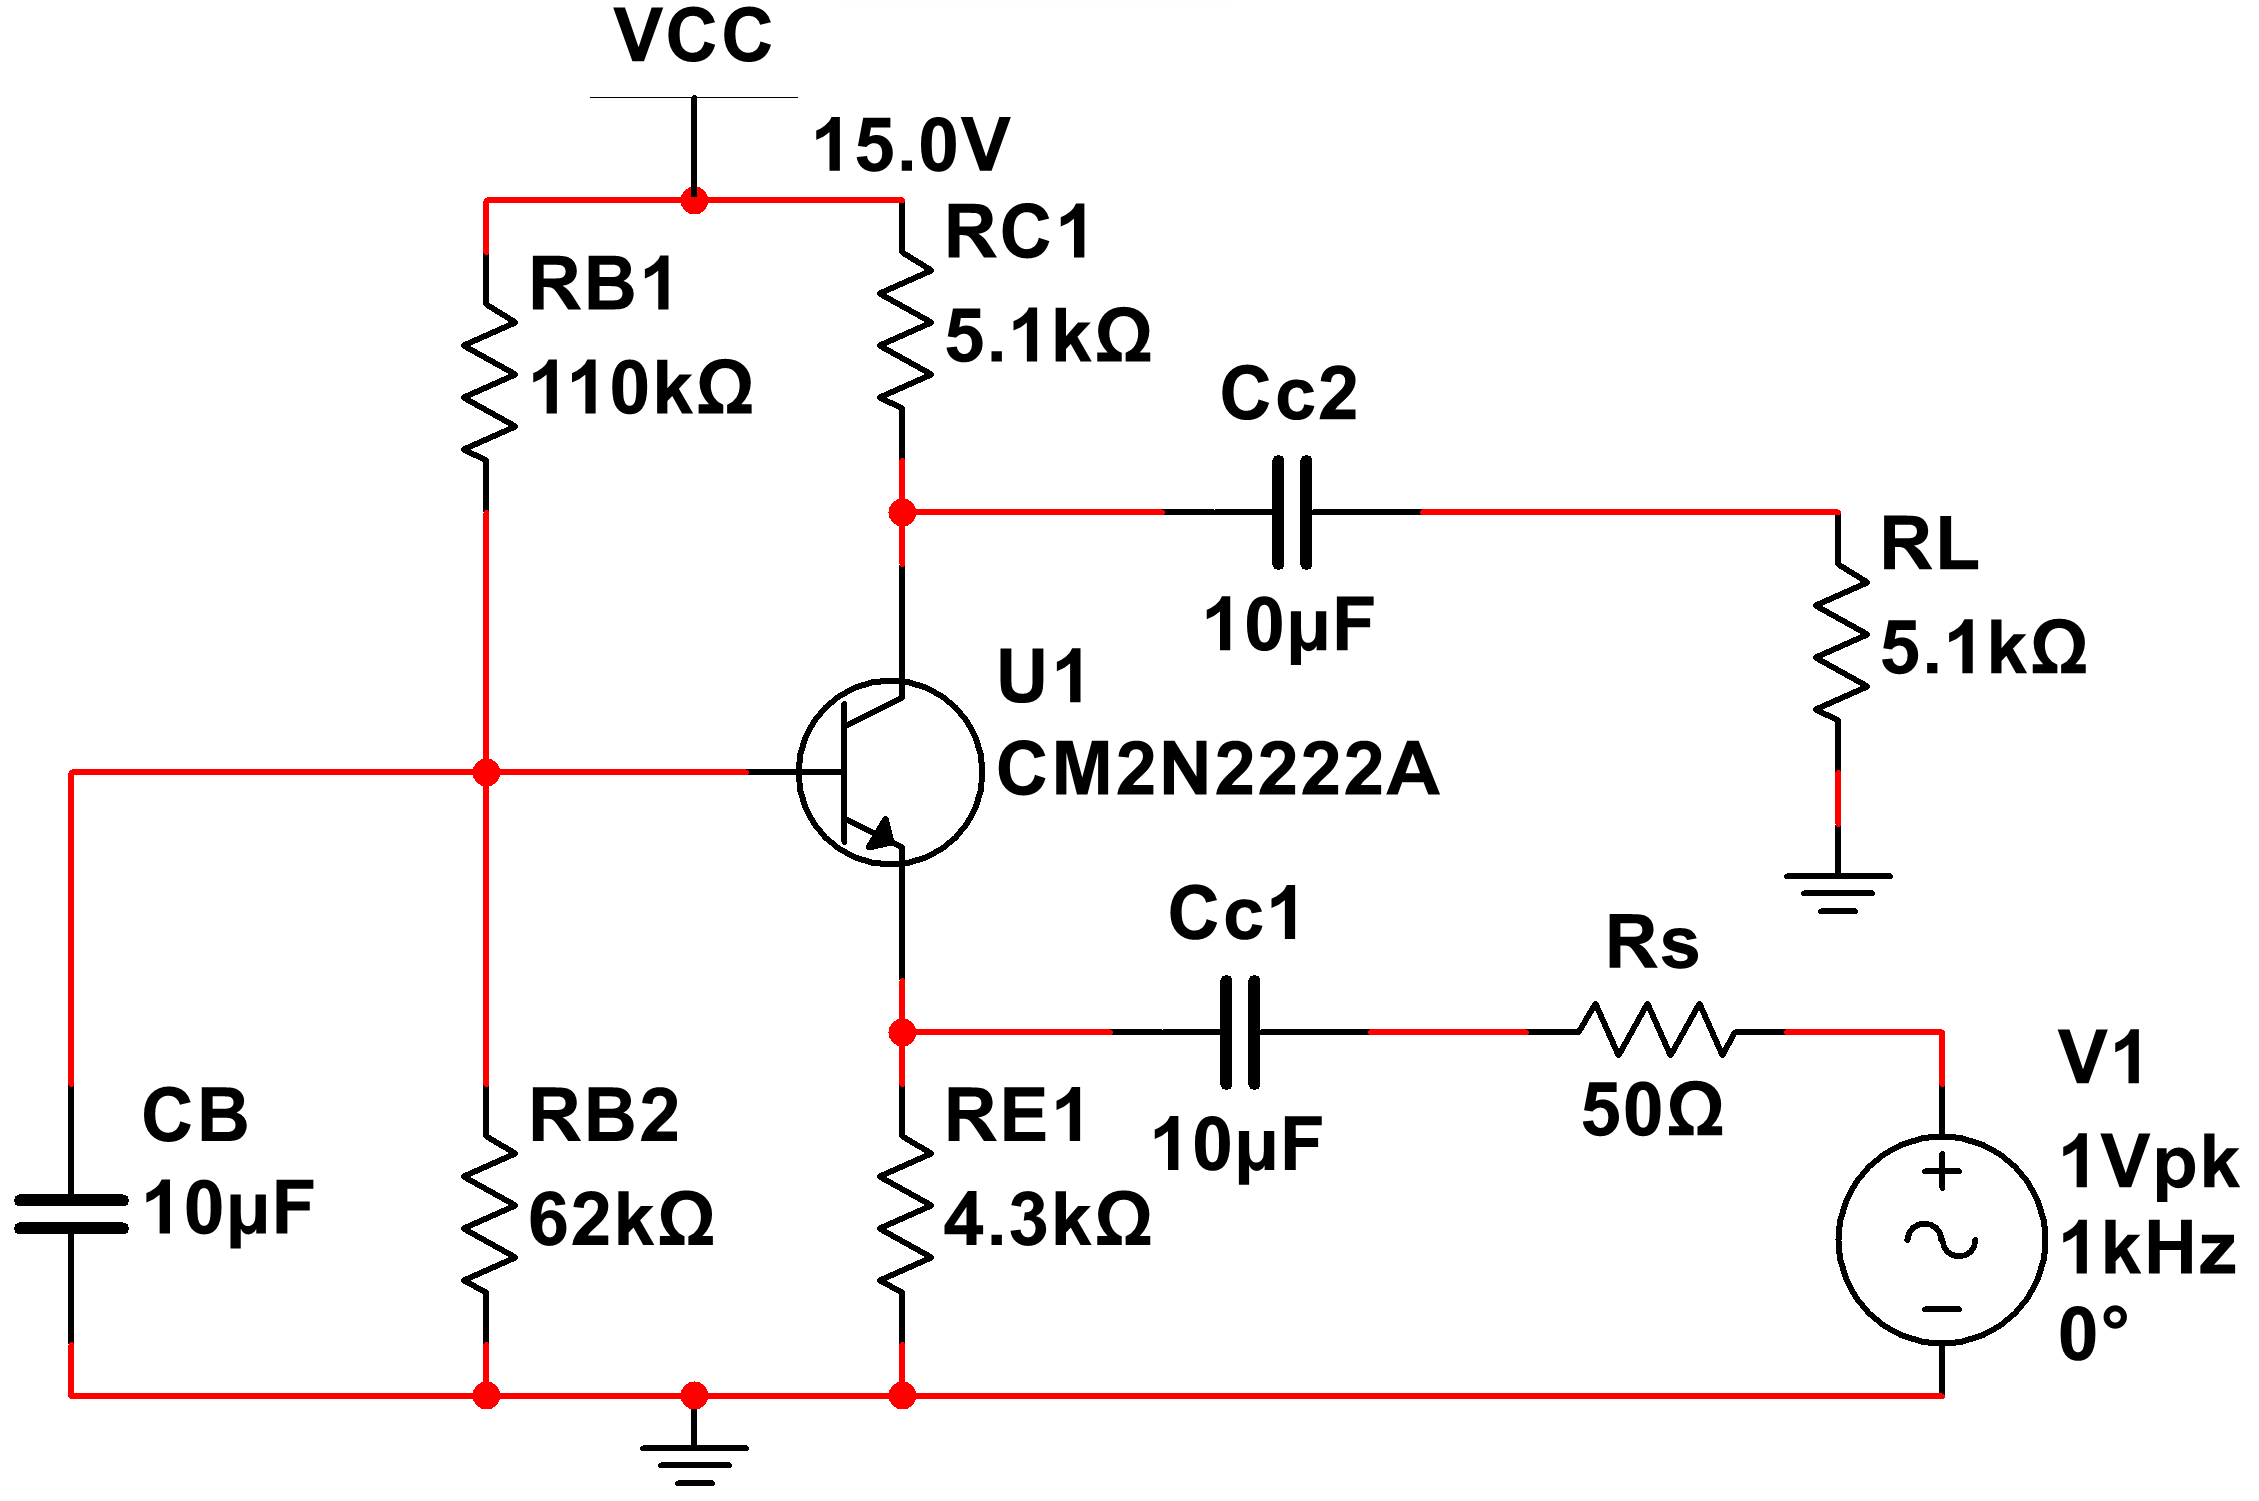
\includegraphics[height=0.40\textwidth]{Images/3acircuit.png}\\
\caption{2N2222A Common Emitter Amplifier}
\label{fig:part3_circuit}
\end{figure}
Here are the bode and phase plots for this circuit:

\begin{figure}[H]
\centering
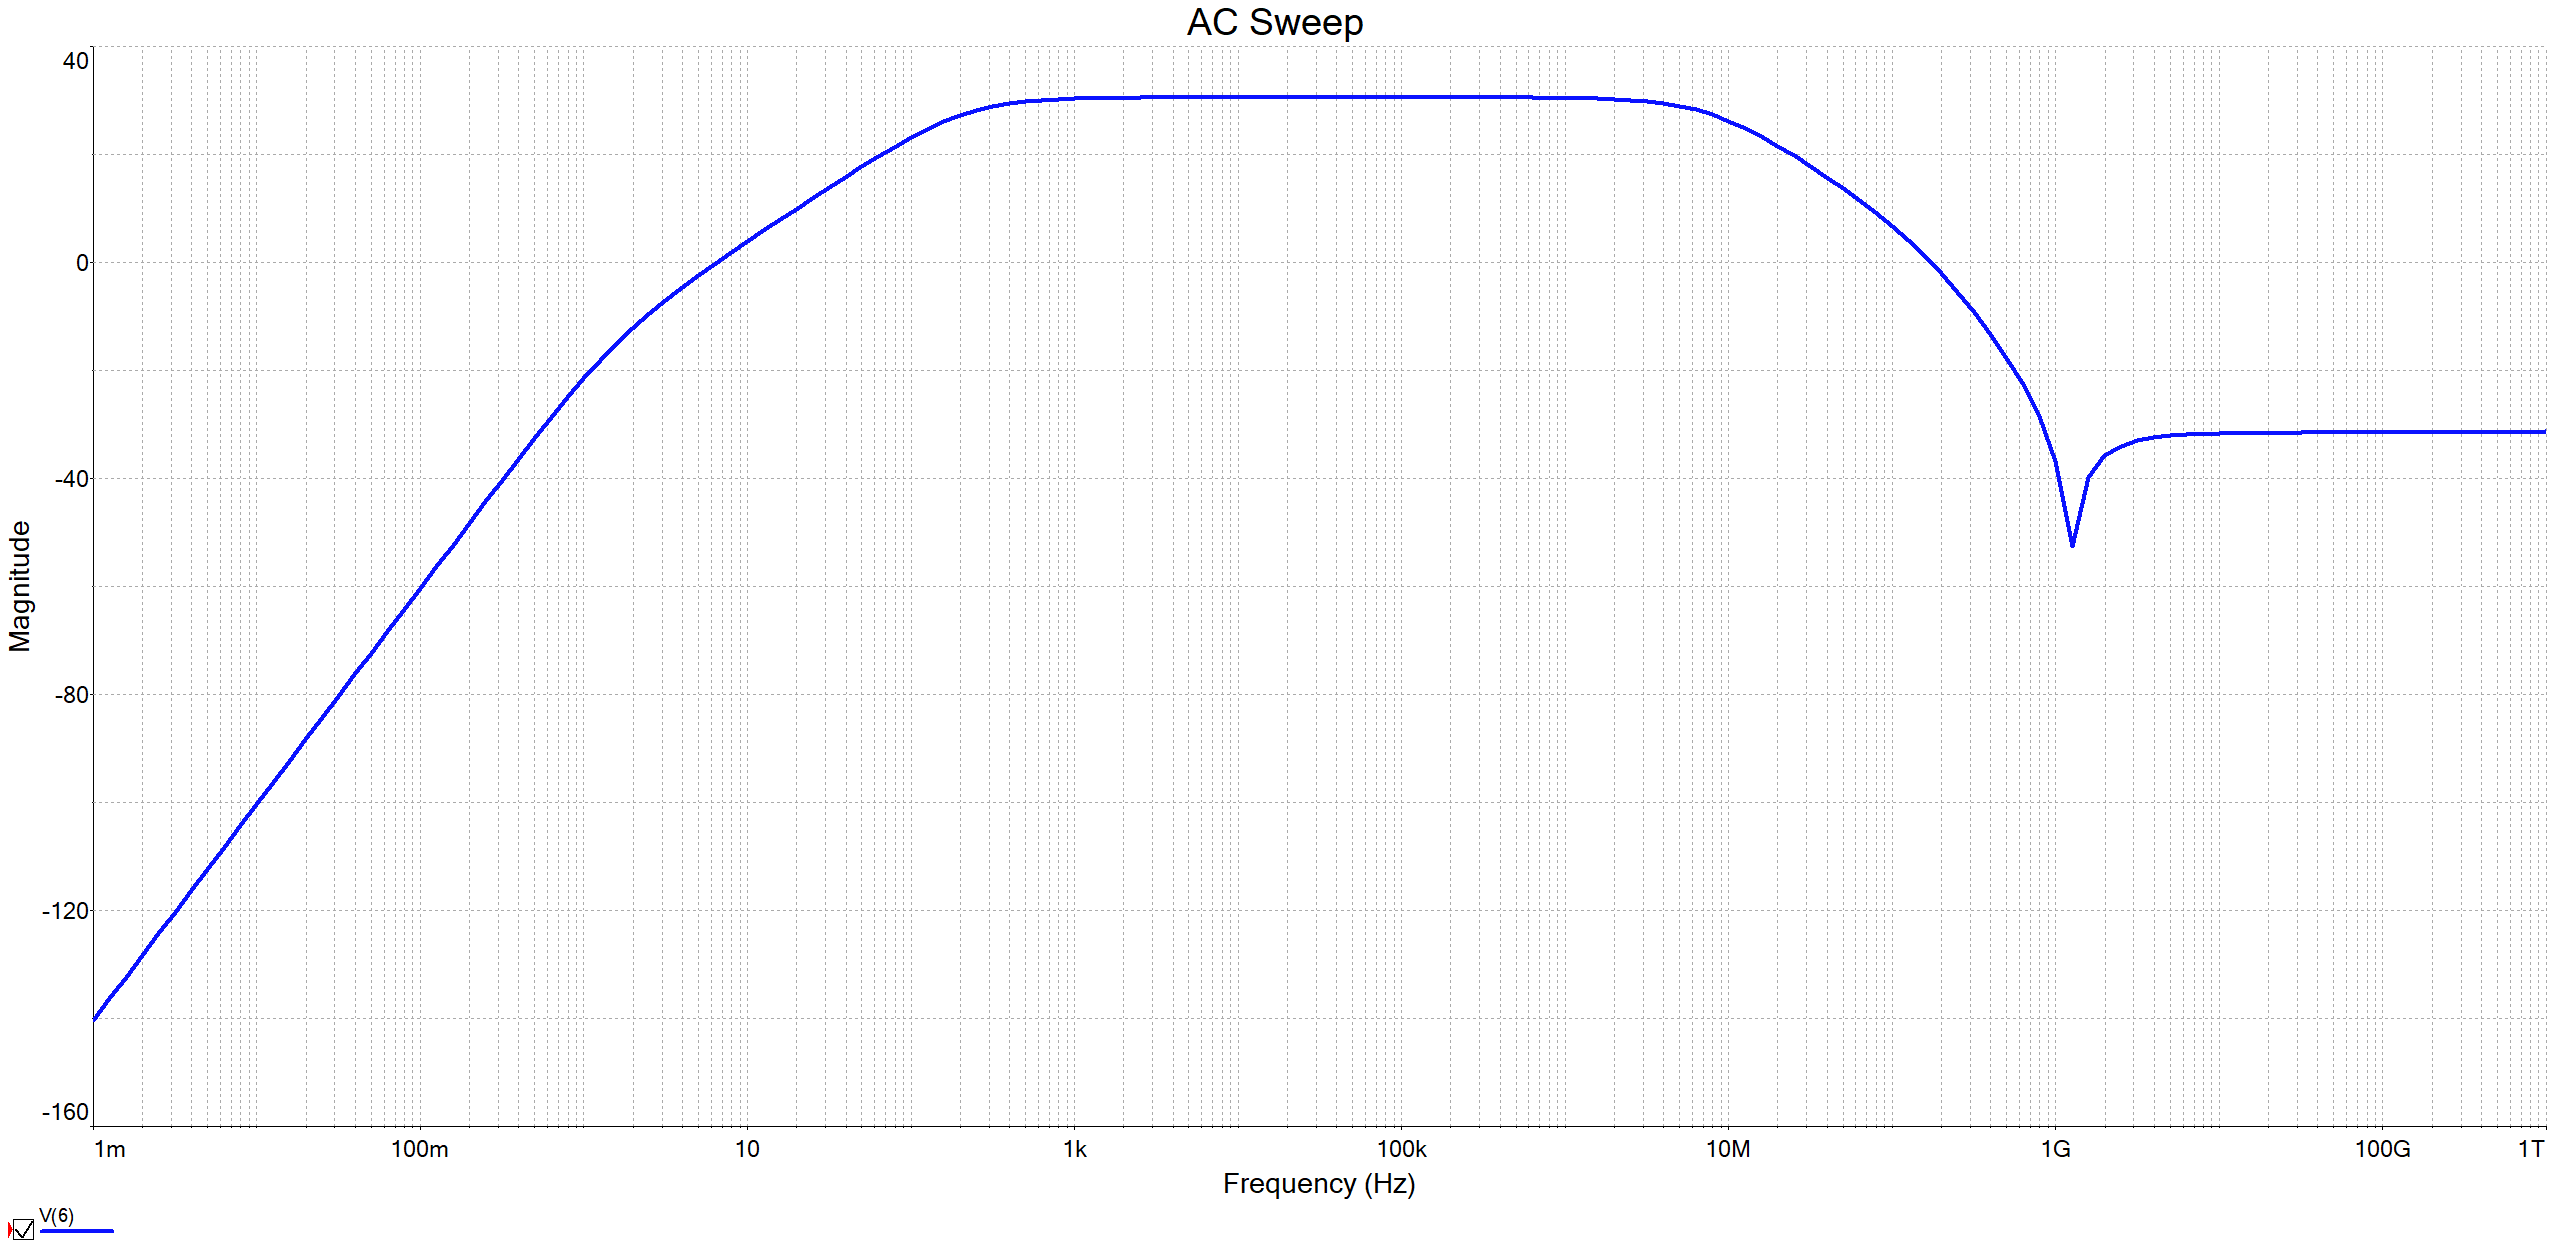
\includegraphics[height=0.45\textwidth]{Images/part3_bode.png}\\
\caption{2N2222A Bode plot}
\label{fig:part3_bodeplot}
\end{figure}
\begin{figure}[H]
\centering
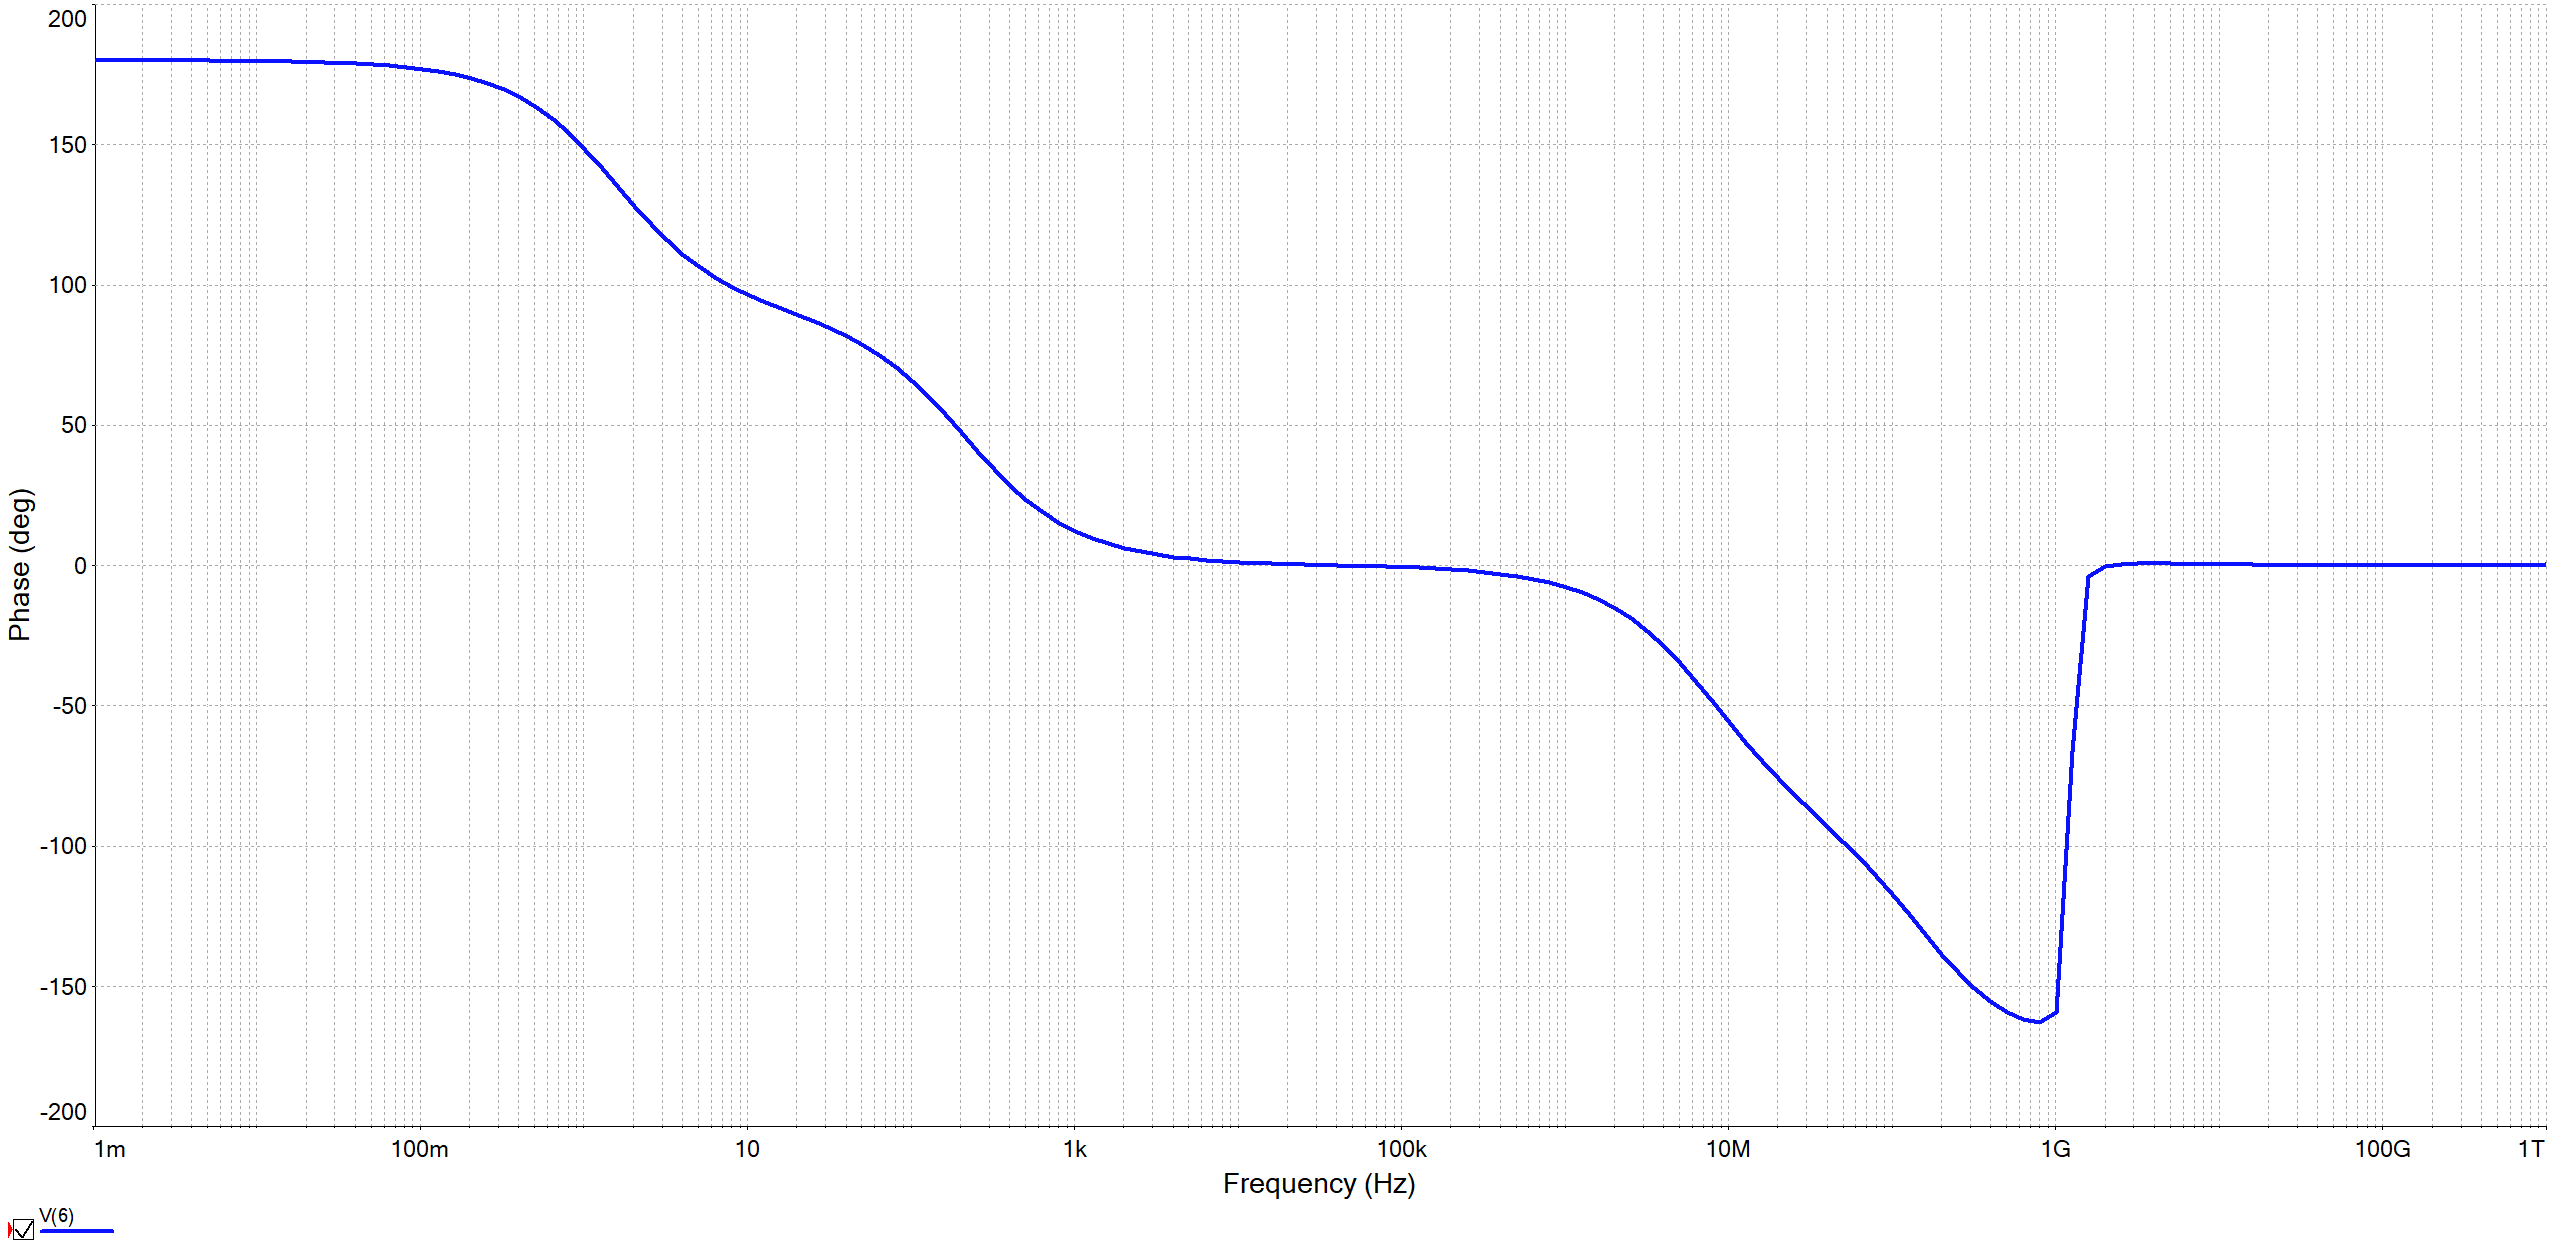
\includegraphics[height=0.45\textwidth]{Images/part3_phase.png}\\
\caption{2N2222A Phase plot}
\label{fig:part3_phaseplot}
\end{figure}

Using the cursors in Multisim$^{TM}$, we are able to approximate our pole and zero values of the bode plot. Here is how we will approximate it:

\begin{figure}[h!]
\centering
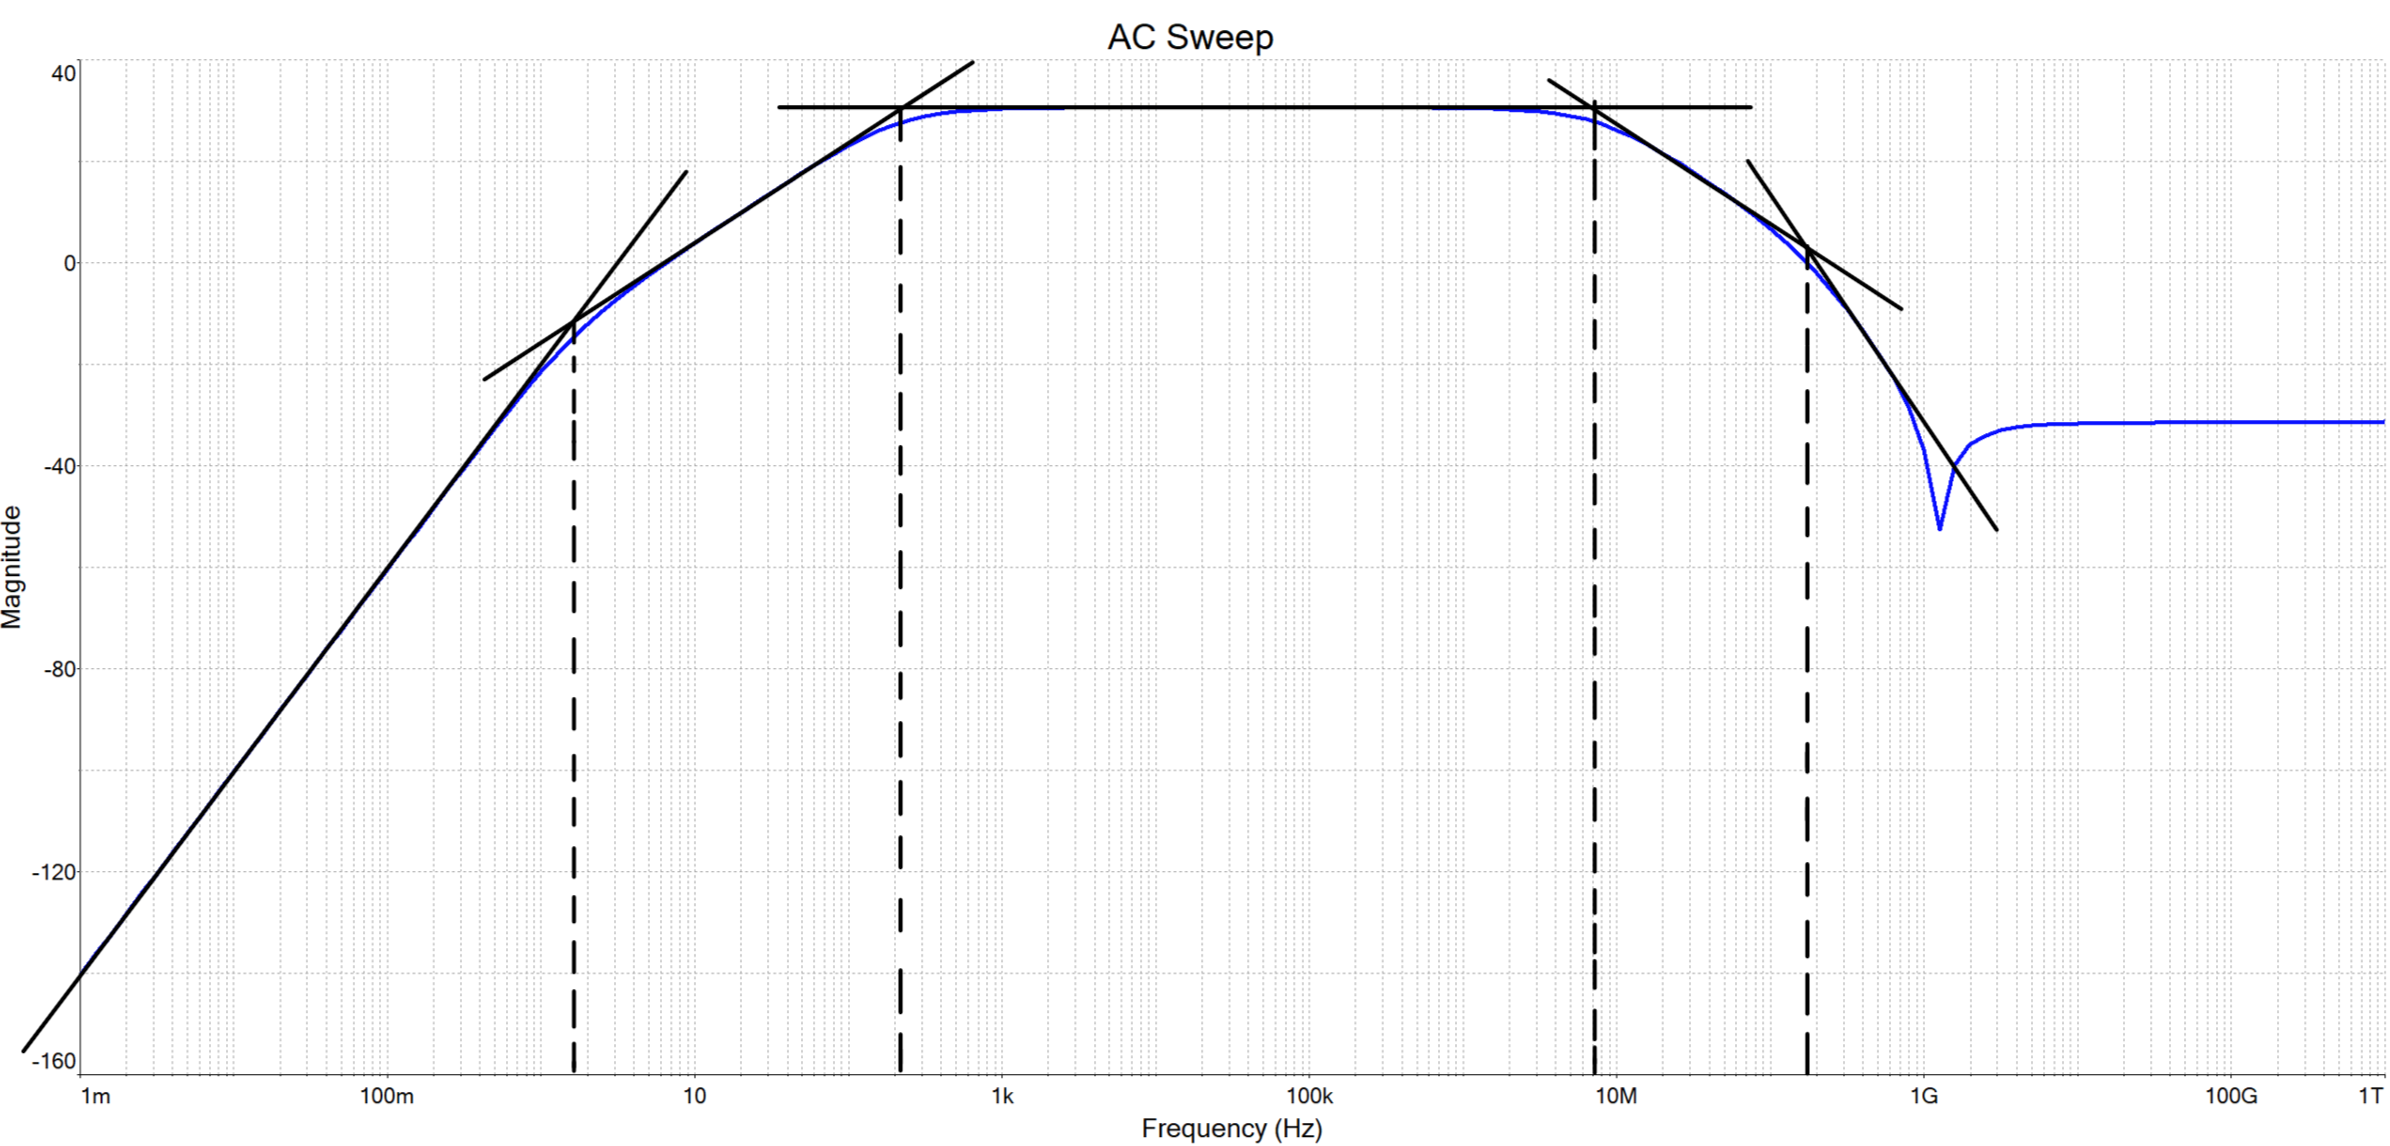
\includegraphics[height=0.45\textwidth]{Images/2abode_approximations_2N2222A.png}\\
\caption{2N2222A Phase plot}
\label{fig:part3_phaseplot}
\end{figure}

Since it is not obvious that there are 3 poles in the lower frequencies, but we know that there has to be 3 poles, we assume that in the approximation that there is a pair of a pole and a zero in the same location.

%---------------Pole approximation and calculations



\begin{table}[h!]
\centering
\begin{tabular}{|l|l|l|l|l|l|l|l|l|}
\cline{1-2} \cline{3-9}
             & $w_{lz1}$ & $w_{lz2}$ & $w_{lz3}$ & $w_{lp1}$  & $w_{lp2}$  & $w_{lp3}$     & $w_{hp1}$          & $w_{hp2}$           \\ \cline{1-2} \cline{3-9}
$w[\frac{rad}{s}]$ &  0    & 0     & 2.721      & 10.903 & 2.721 & 1365.306 & $50.785*10^6$ & $830.207*10^6$ \\
\hline
\end{tabular}
\caption{Table of Approximated Pole Frequencies(2N2222A)}
\label{table:2N2222A_Approximated_Poles}
\end{table}
\begin{table}[h!]
\centering
\begin{tabular}{|l|l|l|l|l|l|l|l|l|}
\cline{1-2} \cline{3-9}
             & $w_{lz1}$ & $w_{lz2}$ & $w_{lz3}$ & $w_{lp1}$  & $w_{lp2}$  & $w_{lp3}$     & $w_{hp1}$          & $w_{hp2}$           \\ \cline{1-2} \cline{3-9}
$w[\frac{rad}{s}]$ &  0    & 0     & 2.522      & 9.804 & 2.659 & 1361.059 & $48.945*10^6$ & $ 827.913*10^6$ \\
\hline
\end{tabular}
\caption{Table of Calculated Pole Frequencies(2N2222A)}
\label{table:2N2222A_Calculated_Poles}
\end{table}
\FloatBarrier
From the pole approximations, we can see that the poles and zeros are close to the calculated values. As we can see, one of the poles are complex. The calculations for the poles and zeros are from the class notes, and listed as no. 3 in the Appendix.
\subsubsection{Part b)}
Here, we will be setting our mid-band frequency to be 100kHz. Plotting $\frac{v_o}{v_s}$, as done previously, we find:

\begin{figure}[H]
\centering
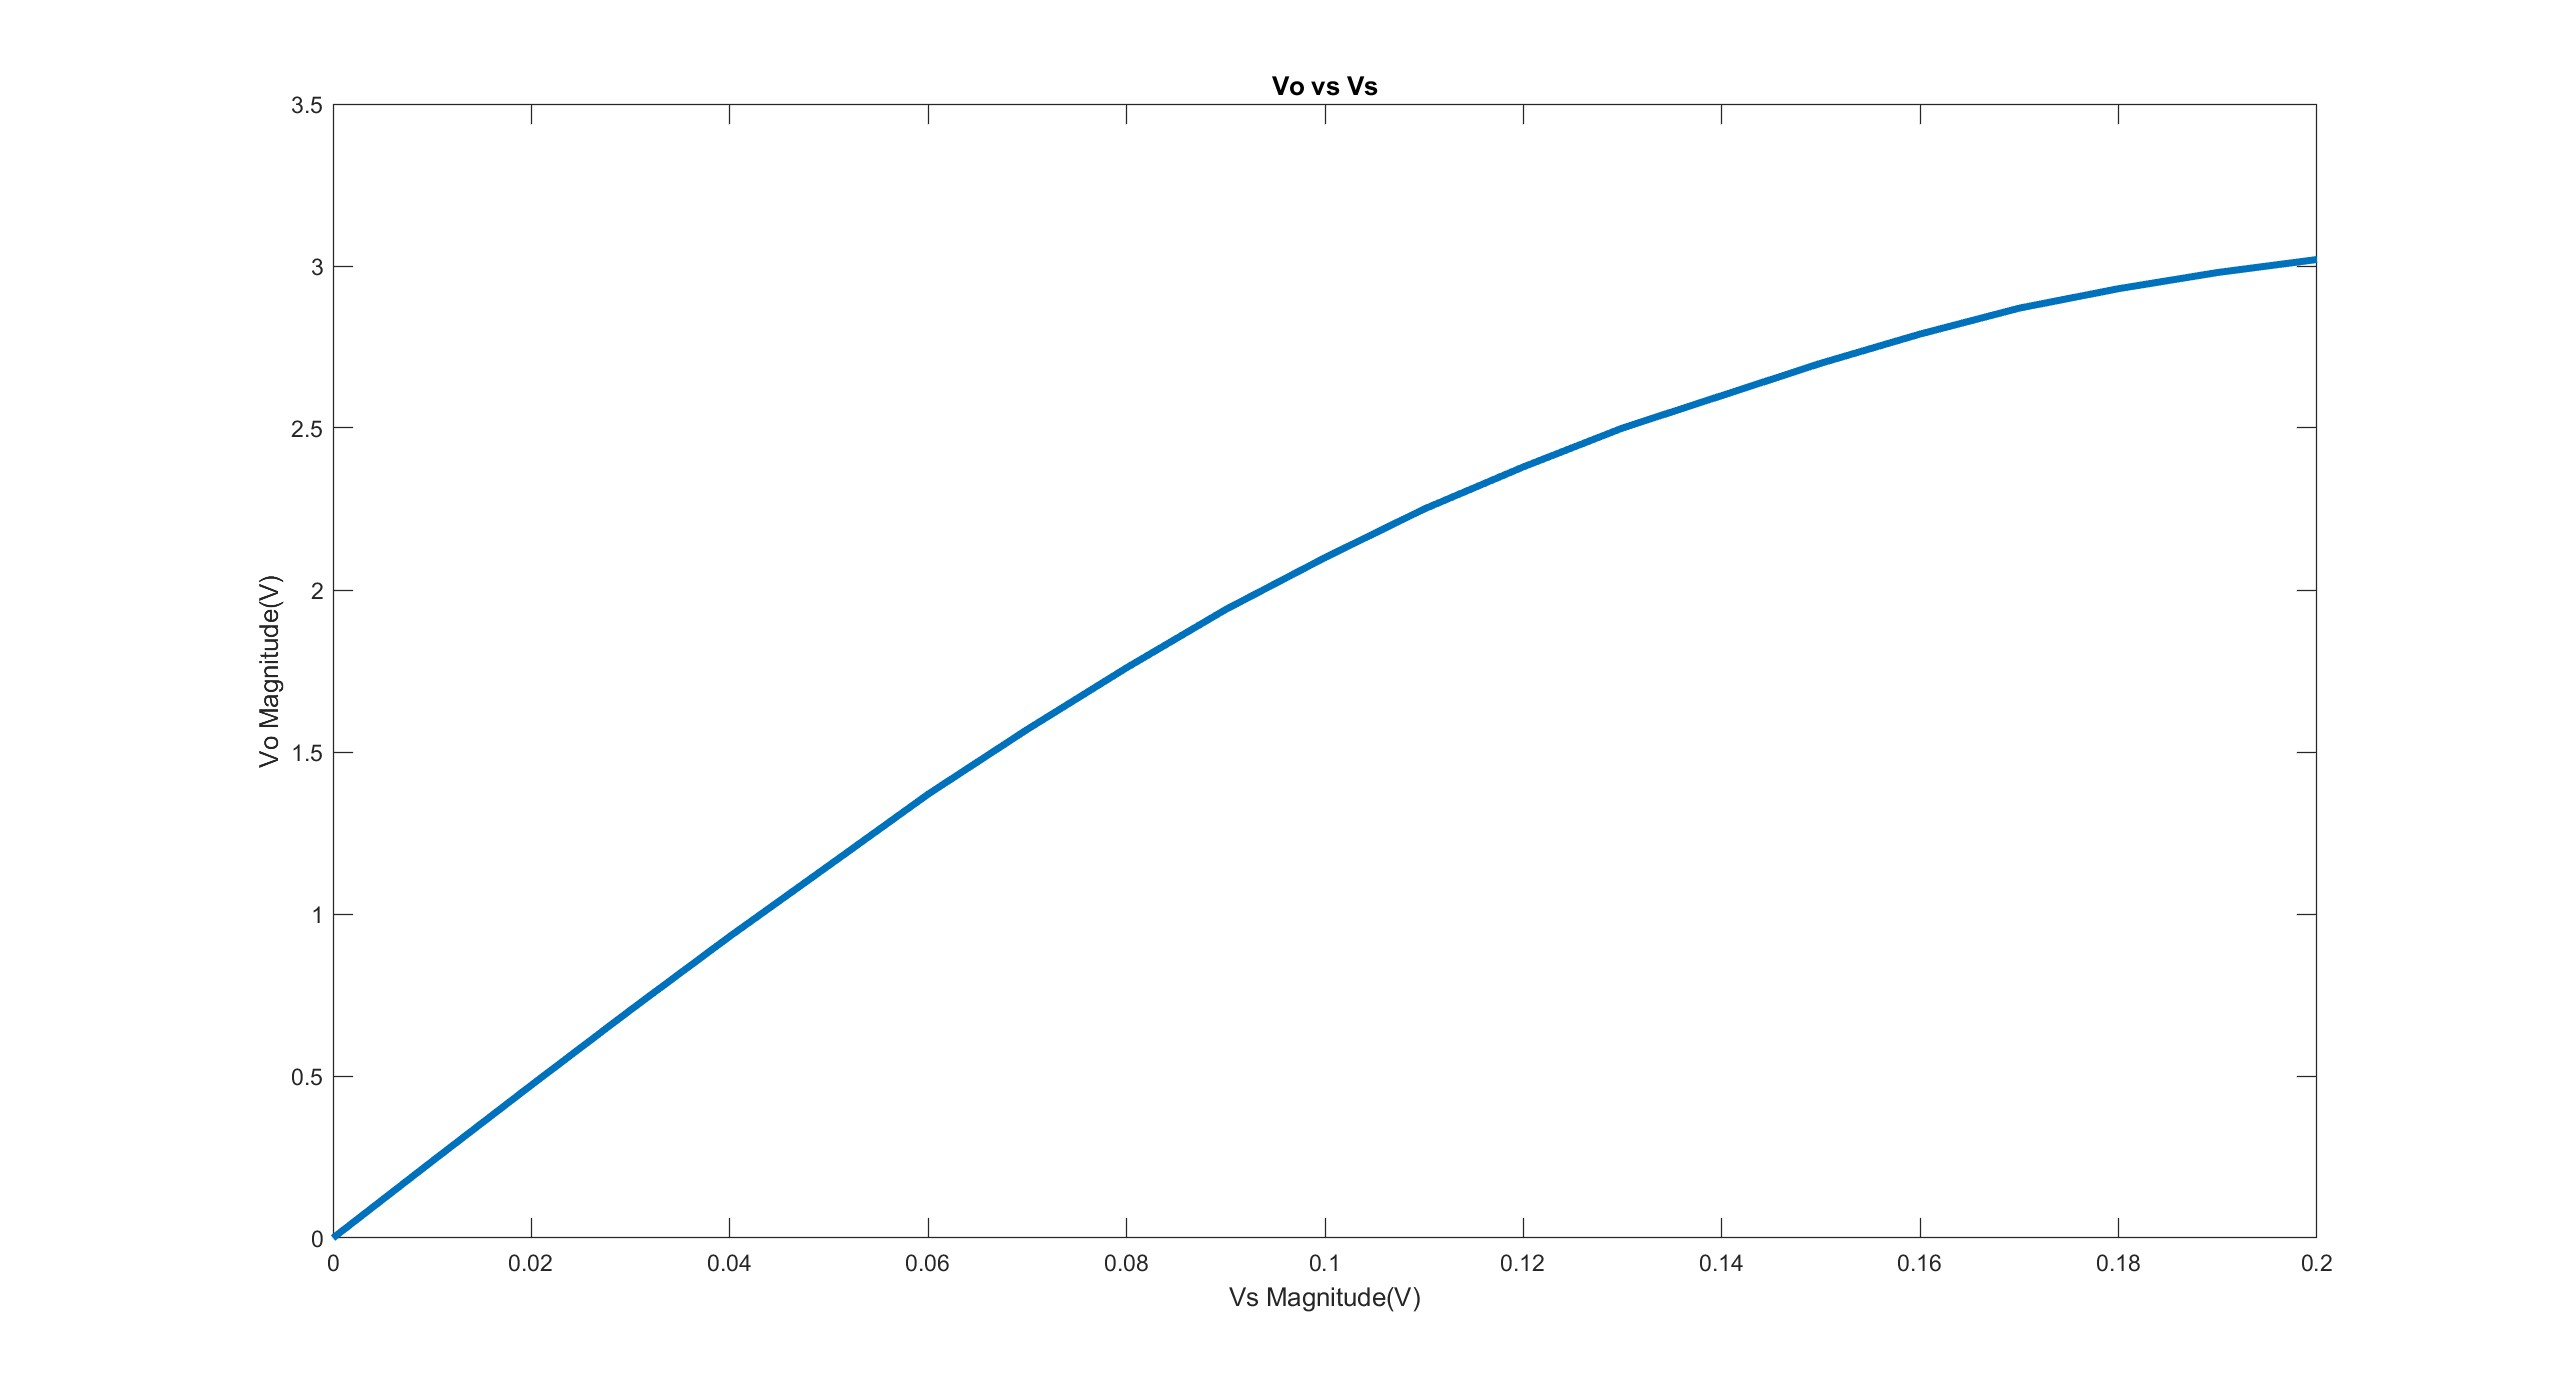
\includegraphics[height=0.5\textwidth]{Images/voltage_transfer_plot_2N2222A.jpg}\\
\caption{$V_o$ vs $V_s$ (2N2222A)}
\label{fig:transfer_plot_2N2222A}
\end{figure}
We are able to observe that the plot begins to be non linear around 0.05V.

\subsubsection{Part c) and d)}

To measure our input and output impedance, we will be using the same procedure as done for the 2N3904 and 2N4401. We will still measure our voltages and currents at the inputs and the outputs to get our input and output impedance. The frequency is still set at 100kHz, and our voltage input amplitude will be set at 0.01V.

\begin{center}
$R_{in}=\frac{2.38mV}{93.8\mu A}$ = \boxed{25.373\Omega}, $R_{out}=\frac{237mV}{46.4\mu A}$ = \boxed{5.107k\Omega}
\end{center}

Our calculation for the input and output impedance is:
\begin{center}
$R_{out}=R_C$= \boxed{5.1k\Omega}, $R_{in}$=\boxed{23.472\Omega}
\end{center}
The calculations for the impedance are from formulas that are covered in the class notes, and is listed in no. 4 in the Appendix. 
As we can observe here, one can see that the calculated impedance is close to the measured impedance.
\section{Conclusion}

To conclude, we have learned how to estimate resistor values for biasing a BJT with the 1/3 rule, estimating pole and zero values, and determining which between two transistors performs better. We can also find that the values calculated from the simulation match with values found in the equivalent transistor data sheet. We have also learned that the approximations of the poles and zeros from the plots are relatively accurate to the calculated values.
\newpage
\section{Appendix}
1. Calculations for finding pole frequencies and zero(CE Amplifier):
\begin{flalign}
&C_{\pi} = 2*CJE+TFg_m\\
&C_{\mu}=\frac{CJC}{(1+\frac{V_{CB}}{VJC})^{MJC}}\\
&w_{zl3}=\frac{1}{R_{E}*C_{E}}\\
&R_{BB}=R_{B1}||R_{B2}\\
&w_{HP1}= \frac{1}{R_{BB}||R_{\pi}||[R_S(C_{\pi}+C_{\mu}(g_m(R_C||R_L)))]}\\
&w_{HP2}=\frac{1}{C_{C2}(R_C+R_L)}\\
&w_{LP1}=\frac{1}{C_{C2}(R_C+R_L)}\\
&w_{LP2}=\frac{1}{C_{C1}[(R_s+R_{BB})||(r_{\pi }+(1+\beta)R_e)]}\\
&w_{LP3}=\frac{1}{RE||\frac{R_{\pi}+R_{BB}}{1+\beta}}\\
\end{flalign}
2. Calculations for Input and Output Impedance(CE Amplifier):
\begin{center}
$R_{in}=R_{BB}||R_{\pi}$, $R_{out}=R_C$
\end{center}
3. Calculations for finding pole frequencies and zero (CB Amplifier):
\begin{flalign}
&C_{\pi} = 2*CJE+TFg_m\\
&C_{\mu}=\frac{CJC}{(1+\frac{V_{CB}}{VJC})^{MJC}}\\
&w_{HP1}=\frac{1}{\frac{r_\pi}{1+\beta}||R_{E}||R_SC_\pi}\\
&w_{HP2}=\frac{1}{R_C||R_Lc_\mu}\\
&w_{LP1}=\frac{1}{(R_C+R_L)C_{C2}}\\
&w_{LP2}=\frac{1}{(R_{BB}||[r_\pi+(1+\beta)R_E])C_B}\\
&w_{LP3}=\frac{1}{(((\frac{r_\pi+R_{BB}}{1+\beta}||R_E)+R_S)C_{C1}}\\
&w_{zl3}=\frac{1}{R_{BB}{C_B}}
\end{flalign}
\newline
4. Calculations for Input and Output Impedance(CB Amplifier):
\begin{center}
    $R_{out}=R_E||\frac{R_\pi}{1+\beta}$, $R_{in}=R_C$
\end{center}
\newpage
\section{References}
\textrm {1. https://www.onsemi.com/pdf/datasheet/2n3903-d.pdf}\\
\textrm{2. NI Multisim Manual}\\
\textrm{3. Chapter 10 and 11 Class Notes}\\
\textrm{4. Standard Resistor and Capacitor Value Sheet (Canvas)}
\end{document}
